% !TEX encoding = UTF-8 Unicode
% !TEX spellcheck = en-US
%%===================================
\documentclass[12pt]{report}
\usepackage[utf8]{inputenc}
\usepackage[a4paper, margin=2.5cm]{geometry}
\usepackage[pdftex]{graphicx}

% Use newlines instead of tabs for separating paragraphs
\usepackage{setspace}
\doublespacing
\usepackage[parfill]{parskip}

\pdfcompresslevel=9

\usepackage[toc, acronym]{glossaries}
\makeglossaries
% !TEX encoding = UTF-8 Unicode
%!TEX root = thesis.tex
% !TEX spellcheck = en-US
%%=========================================

% !!!!!!!!!!!!!!!!!!!!!!  IMPORTANT    !!!!!!!!!!!!!!!!!!!!!!!!!!!!!!!!!!!!! %
% Remember to clear the cache after updating this, as it otherwise wont work %
% !!!!!!!!!!!!!!!!!!!!!!  IMPORTANT    !!!!!!!!!!!!!!!!!!!!!!!!!!!!!!!!!!!!! %

\newacronym{api}{API}{Application programming interface}
\newacronym{ci}{CI}{Continuous Integration}
\newacronym{cms}{CMS}{Content Management System}
\newacronym{cto}{CTO}{Chief Technology Officer}
\newacronym{devops}{DevOps}{Development and Operations}
\newacronym{dht}{DHT}{Distributed Hash Table}
\newacronym{dry}{DRY}{Don't Repeat Yourself}
\newacronym{ects}{ECTS}{European Credit Transfer and Accumulation System}
\newacronym{html}{HTML}{HyperText Markup Language}
\newacronym{http}{HTTP}{HyperText Transfer Protocol}
\newacronym{iec}{IEC}{International Electrotechnical Commission}
\newacronym{ietf}{IETF}{Internet Engineering Task Force}
\newacronym{ip}{IP}{Internet Protocol}
\newacronym{iso}{ISO}{International Organization for Standardization}
\newacronym{json}{JSON}{JavaScript Object Notation}
\newacronym{mvc}{MVC}{Model-view-controller}
\newacronym{nltk}{NLTK}{Natural Language Toolkit}
\newacronym{ntnu}{NTNU}{Norwegian University of Science and Technology}
\newacronym{rest}{REST}{Representational state transfer}
\newacronym{rfc}{RFC}{Request For Comments}
\newacronym{rps}{RPS}{Requests Per Second}
\newacronym{soap}{SOAP}{Simple Object Access Protocol}
\newacronym{soa}{SOA}{Service Oriented Architecture}
\newacronym{tdd}{TDD}{Test-driven Development}
\newacronym{trk}{TRK}{Trondheim kommune (Trondheim Municipality)}
\newacronym{ui}{UI}{User Interface}
\newacronym{url}{URL}{Uniform Resource Locator}
\newacronym{ux}{UX}{User eXperience}
\newacronym{vm}{VM}{Virtual Machine}
\newacronym{vcs}{VCS}{Version Control System}
\newacronym{wip}{WIP}{Work In Progress}
\newacronym{wsdl}{WSDL}{Web Services Description Language}
\newacronym{wysiwyg}{WYSIWYG}{What You See Is What You Get}
\newacronym{xml}{XML}{eXtensible Markup Language}

% !!!!!!!!!!!!!!!!!!!!!!  IMPORTANT    !!!!!!!!!!!!!!!!!!!!!!!!!!!!!!!!!!!!! %
% Remember to clear the cache after updating this, as it otherwise wont work %
% !!!!!!!!!!!!!!!!!!!!!!  IMPORTANT    !!!!!!!!!!!!!!!!!!!!!!!!!!!!!!!!!!!!! %

\usepackage{fourier}
\pagestyle{headings}
\usepackage{setspace}
\linespread{1.25}

\usepackage{booktabs}
\usepackage{url}
\usepackage{float}

\usepackage{titlesec}

\usepackage{float}
\usepackage{xcolor}
\usepackage{svg}
\usepackage{csvsimple}

\usepackage{marvosym}
\usepackage{rotating}

\usepackage{natbib}
%\usepackage[square]{natbib}
%\usepackage{url}
%\def\UrlBreaks{\do\/\do-}
%\usepackage{breakurl}
%\usepackage[breaklinks]{hyperref}


\usepackage{amsmath}

\usepackage{booktabs}
\usepackage{tabularx}
\usepackage{array}

\usepackage{tikz}
\usetikzlibrary{arrows,positioning,calc,shapes,fit}
\usepackage{pgf-umlsd}
\usepackage{pgfplots}
\pgfplotsset{compat=1.13}
\usepackage{xargs} % uses more than one argument in new commands


%\usepackage[colorinlistoftodos,prependcaption]{todonotes} % Write \usepackage[disable]{todonotes} to temporarily remove all notes
\usepackage[disable]{todonotes}

\newcommandx{\unsure}[2][1=]{\todo[linecolor=red,backgroundcolor=red!25,bordercolor=red,#1]{#2}}
\newcommandx{\change}[2][1=]{\todo[linecolor=blue,backgroundcolor=blue!25,bordercolor=blue,#1]{#2}}
\newcommandx{\info}[2][1=]{\todo[linecolor=OliveGreen,backgroundcolor=OliveGreen!25,bordercolor=OliveGreen,#1]{#2}}
\newcommandx{\improvement}[2][1=]{\todo[linecolor=purple,backgroundcolor=purple!25,bordercolor=purple,#1]{#2}}
\newcommandx{\thiswillnotshow}[2][1=]{\todo[disable,#1]{#2}}


\newenvironment{remark}{\par\mbox{}\par\noindent{\bfseries \emph{Remark}\/}:\normalfont}{\par}
\newenvironment{defin}{\par\mbox{}\par\noindent\bfseries \emph{\Pointinghand\ }\normalfont}{\par}
\setcounter{tocdepth}{2} 

\usepackage[colorlinks=true, pdfstartview=FitV,
linkcolor=black, citecolor=black, urlcolor=blue]{hyperref}
\setlength{\topmargin}{-10mm}

\usepackage[tableposition=top]{caption}  % Make captions be on top of tables with some vertical spacing too


%%===================================
\begin{document}
% !TEX encoding = UTF-8 Unicode
%!TEX root = thesis.tex
% !TEX spellcheck = en-US

%This is the Titlepage
%%=========================================
\thispagestyle{empty}
%\includegraphics[scale=1.1]{fig/rams}

\includegraphics[scale=0.7]{fig/NTNU}
\mbox{}\\[6pc]

\begin{center}

%\todo[inline]{Figure out if we should give it a new title which doesn't have any abbreviations 
%%{[}Prio: Low{]} }
\textbf{\Huge{
Developing a Content Management System with a Microservice Architecture
}}\\[5pc]

\if 
Developing a Microservice Based \\ Content Management System
Developing a Content Management System with a Microservice Architecture
CMS using Microservices \\
Exploring Microservices\\
Microservice; A proof of concept
\fi


\large{Group 1}\\
\small{
Aleksander Hansen\\
Haakon Johansen Jonsson\\
Pål Karlsrud\\
Ole Martin Knurvik\\
Nicklas Grimstad Nilsen\\
Håkon Larsen Solbjørg\\
\textit{Thomas Hansen (Dropped out 7th of March)}\\
}
\vspace{35mm} %35mm vertical space
\large{May 2016}\\[2pc]
\small{Department of Computer and Information Science}\\
\footnotesize{Norwegian University of Science and Technology}
\end{center}
\vfill

\noindent \textbf{Professor:} Monica Divitini \\
\noindent \textbf{Supervisor:} Katja Abrahamsson \\
\noindent \textbf{Client:} Mohsen Anvaari, Trondheim Municipality
 % This is the titlepage
\newcounter{savepage}  %% Creates a counter for saving the roman page counter
\setcounter{page}{0}
\pagenumbering{roman}
% % !TEX encoding = UTF-8 Unicode
%!TEX root = thesis.tex
% !TEX spellcheck = en-US
%%=========================================
\addcontentsline{toc}{section}{Acknowledgment}
\section*{Acknowledgment}
I would like to thank the following persons for their great help during \ldots

If the project has been carried out in cooperation with an external partner (e.g., a company), you should acknowledge the contribution and give thanks to the involved persons.

You should also acknowledge the contributions made by your supervisor(s).

\begin{flushright}
O.N.\\[1pc]
(Your initials)
\end{flushright}
% % !TEX encoding = UTF-8 Unicode
%!TEX root = thesis.tex
% !TEX spellcheck = en-US
%%=========================================
\chapter{Summary and Conclusions} %% Summary, reflection, conclusion, yo dawg dis happened.
\label{chapterSummary}

%% THE FOLLOWING COMMENT IS REGARDING MASTER THESIS' AND SHOULD BE TREATED AS SUCH 
%% Here you give a summary of your your work and your results. This is like a management summary and should be written in a clear and easy language, without many difficult terms and without abbreviations. Everything you present here must be treated in more detail in the main report. You should not give any references to the report in the summary -- just explain what you have done and what you have found out. The Summary and Conclusions should be no more than two pages.

%% You may assume that you have got three minutes to present to the Rector of NTNU  what you have done and what you have found out as part of your thesis. (He is an intelligent person, but does not know much about your field of expertise.)

\section{Architecture}
\subsection{Architectural advantages}
In developing microservices, separation of responsibilities as a guiding principle has resulted in benefits like reuse of code and modularity. This is a notable advantage over other architectures, such as Server-Client and \acrlong{soa}. 
Server-Client architectures are generally monolithic, and over time in a production environment they grow unwieldy as new features are added, and old features are hard to replace without extensive code refactoring, because of internal backwards-compatibility.

\acrlong{soa} is an older architecture than microservices, though is in a way similar. Nevertheless, \acrshort{soa} has unclear and varying definitions and the architecture does not have the same overall guideline of separation of responsibilities as the microservice architecture. This leads to \acrshort{soa} often growing monolithic, as the responsibilities of each service grows, rather than being split into more services like with the microservice architecture.  

\subsection{Architectural disadvantages}
A complication with the microservice architecture is the separation of responsibilities. The group spent a while deciding which microservices to implement, and even throughout the project decisions were changed, as with the search service. 

Microservices, having large degrees of separation, also incur some communication overhead when using the exposed functionalities of each other. A related problem to this is how to share information that is common among services, without having redundancies. The group decided to give each service that needed one its own database, even though this incurred penalties with regards to redundancy. This was to ensure modularity and not having a service being replaced affect other services usage of stored data to a large extent. 

\section{Problems and solutions} 

\subsection {Time schedule}
\label{sub:timeSchedule}
Figure \ref{fig:wednesday} illustrates a typical Wednesday from 8:00 to 16:00, where a check mark indicates the team member being available, while unchecked indicates unavailable. Each row represents a team member. Most of the days in a week, including weekends, looked somewhat like this. The combined time schedules made it very hard to have regular meetings. Monday and Thursday afternoon were the only options which suited the entire group throughout most of the semester. Therefore all meetings with the client and supervisor were scheduled for these time slots. 

\begin{figure}[H]
    \centering
    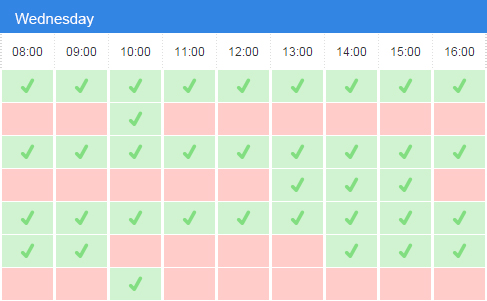
\includegraphics[scale=0.70]{fig/summary/wednesday}
    \caption{Example of our schedule. One row for each team member.}
    \label{fig:wednesday}
\end{figure}


\subsection{Abroad}
\noindent One of the group members had a part-time job in London the first half of the semester. This did not help the already troublesome schedule crash.
In addition, there was an excursion in March that three of the members were attending. This all meant a way of having stand-up meetings and exchanging information more frequently than the two meetings a week was needed. Geekbot was chosen for arranging online stand-up meetings. Communication is detailed in section \ref{sectionCommunicationTools}.

\subsection{Group member leaving}
At the beginning of the second iteration, a group member had to leave the course and the project for personal reasons. This meant that the group would go from seven people, down to six. The group worked around this by reassigning the workload to the remaining members. This announcement happened at a less unfortunate time, as the tasks for the second sprint had not yet been fully decided upon; planning for a six person group was relatively easy. 

This could of course have become problematic later on in the project if the total workload was larger than the reduced team could handle. Keeping in mind that the customer was more interested in a demonstration than the product features, scaling down functional requirements accordingly did not concern the customer much.

\section{Lessons learnt}

\subsection{Project organisation}

\paragraph{Schedules} Matching schedules is not a necessity for a project to succeed, but it makes the job a whole lot easier. Through planning and different tools, the problems were simplified, but with more similar schedules this could have been avoided in the first place. 

\paragraph{Development method} Looking back at the project, starting out with a more defined development method would have been beneficial and saved us some time. Agile development methods like Scrum work better when the team has a common background regarding development tools and how to use them. Digital Scrum boards, stand-up meetings, and other elements take time to learn and accustom to, and thus often benefit less than the required time investment for small projects.

\paragraph{Meetings} Even though it was not a huge problem, having more frequent meetings and work sessions would have improved the overall progression of the project early on. 

\subsection{Development}

\paragraph{Tools and frameworks} Learning to use tools and frameworks not familiar to the team may take more time than first anticipated. Thus, one should try to mostly use tools people are familiar with, unless the tool is required and there are no familiar alternatives.

\paragraph{Status} The status service could contain a cache of documentation and check if a newer version is available, to make sure documentation for a service is available even if the service is unavailable.

\paragraph{Front-end} The implemented front-end of the system is a bit too tightly coupled to be a true microservice. By splitting it up, or having different services provide their own front-end, this could have been achieved. This would require more work, despite being a nice possible addition to the project. 

\section{Conclusion}
The project started with some difficulties due to absence of one of the team members. This was handled by selecting an appropriate tool to facilitate team communication. This turned out to work quite well and had no major impact on the work flow. The roles and responsibilities of each team member were settled in a natural way, as each team member took on tasks that had been prioritised by the team. As the project evolved the different sub-teams worked on their part of the project and reported on the status during the weekly meetings. During the meetings people had the opportunity to share information and seek help on any problems encountered. 

Communication with the customer has been good overall, even though some more preparations could have been done beforehand by the team. All in all the project went smoothly and no major problems were encountered. 
%Any problems encountered along the way was taken care of in an efficient and effective way by the team, making the whole experience informative and interesting.

Even though the system is only a demonstration of microservices, it is a possibility that a third party might be interested in continuing working on the project. Therefore, steps have been taken to ensure that future developers can easily continue on the project if needed. The \acrshort{api} for every applicable microservice has been documented, so the services are easy to work with. If creating a replacement for a microservice is desirable, it is easy to find out which features require being implemented. A setup guide has been created to make it easy to deploy a new instance of the system. There are also tests for the services that can be used to validate future changes and make sure the system remains stable.

% forslag til oppsummerende setning: All in all the group felt that the requirements and goal defined at the start of the project ...somthing something ..

\section{Summary}

The project originated in the customer's expressed desire for a system implementation using microservices.
The group, through this project having implemented such a system, has to a large degree noticed many of the advantages that microservices are purported to have, which reflects many of the customer's hopes and expectations. %JA?
Overall, we feel that the requirements and goals outlined have been achieved to a satisfactory degree.


%!TEX encoding = UTF-8 Unicode
%!TEX root = thesis.tex
%!TEX spellcheck = en-US
%%=========================================

\addcontentsline{toc}{section}{Abstract}
\section*{Abstract}
\label{chapterAbstract}
%Here, you give a brief introduction to your work. What it is (e.g., a Master's thesis in RAMS at NTNU as part of the study program xxx and\ldots), when it was carried out (e.g., during the autumn semester of 2021). If the project has been carried out for a company, you should mention this and also describe the cooperation with the company. You may also describe how the idea to the project was brought up.

%You should also specify the assumed background of the readers of this report (who are you writing for).\\[2cm]

A thesis for the Bachelor in Informatics study program at NTNU, with the goal of demonstrating the usage of microservices for Trondheim Municipality. The thesis was completed during spring 2016.

The client, Trondheim Municipality, is 
as of spring 2016 using multiple monolithic systems. In contrast, Oslo Municipality is actively expanding infrastructures into microservices \citep{osloMicroservices}.
The use of microservices aids in simplifying maintenance, accelerates development of new features and enables ad-hoc repair of software defects without bringing down entire systems. 

The project purported to implement a demonstration of a Content Management System for Trondheim Municipality, using a microservice architecture. A monolithic implementation was ordered from an external company by Trondheim Municipality prior -- the microservice implementation being an exploration into a a potentially more advantageous solution.



\hypersetup{linkbordercolor=black}
\hypersetup{linkcolor=black}


%%=========================================
% Table of ...
\tableofcontents
\addcontentsline{toc}{section}{\listfigurename}
\listoffigures
\addcontentsline{toc}{section}{\listtablename}
\listoftables
\listoftodos
%%=========================================
%  Acronyms   %% move this to beginning
\printglossary[type=\acronymtype]
\printglossary
\clearpage
%%=========================================
\setcounter{savepage}{\arabic{page}}  %% Remember the roman pages before changing to arabic
\pagenumbering{arabic}

%%=========================================
% Chapters
%!TEX encoding = UTF-8 Unicode
%!TEX root = thesis.tex
%!TEX spellcheck = en-US
%%=========================================
\chapter{Introduction}
\label{chapterIntroduction}

This project is a part of IT2901 - Informatics Project II. The course aims to teach about process and organisation in software development projects. The course grants 15 credits (\acrshort{ects}) and serves as the bachelor assignment for Informatics bachelor degrees at \acrshort{ntnu}.

Students partaking in the course were divided into groups and assigned an actual customer, who provided a project to be developed and documented by the students -- this report being the documentation of the development of a Content Management System using microservices made for the municipality of Trondheim.

The report was written for the faculty staff and the customer. It contains some terminology assumed known to the reader. Acronyms, abbreviations, and some terms used are listed in the acronyms section.

\section{Customer} \label{section:introductionCustomer}
Trondheim Municipality, with around 13 000 employees, delivers various services to its employees and to the citizens of the municipality through construction, roads, education, health care, environment, politics, and cultural domains. An ever-growing set of these services have been and are in the process of being digitised. New services are intended to be web- and app based solutions, and to be highly integrated with each other in an attempt to reduce information redundancy and increase reusability.

As an architecture principle, all new systems in \acrshort{trk} should be developed based on the \acrshort{soa}-pattern.
However, \acrshort{soa} is in the process of changing its paradigm from a monolithic structure to a microservice structure.
The microservice concept has, as of 2016, been the subject of numerous heavy discussions with advocates on both sides. % "both sides" as in opponent/proponent. Is this clear from the context?

Microservices are however not only a theoretical concept. Oslo Municipality is one of the adopters of this concept, and has developed around 150 microservices \citep{osloMicroservices}. Trondheim Municipality is interested in seeing how a microservice oriented system functions compared to a monolithic system.

\acrshort{trk}s new \acrshort{cms} ordered from an external customer will be a monolithic system. In this proof-of-concept project, there was expressed desire to see how a microservice \acrshort{cms} developed by IT2901 students would perform regarding time-to-market, performance, modularity, and scalability \citep{trkInfo}.

\section{The team}
The team consists of six students at \acrshort{ntnu}, all of whom are on their final year of a bachelor's degree in informatics. All have different knowledge and expertise within informatics due to different backgrounds and many elective courses in the degree. This results in a very broad field of knowledge, which is useful to the project and can be used to aid in internal knowledge transfers for faster learning and productivity. 


\section{The project goal}
The main purpose of the project is to create a working system using a microservice architecture. Due to the project being a demonstration of an architecture, it is important to prioritise displaying the benefits of the architecture, as well as revealing potential disadvantages and possible solutions and workarounds.
As such, the \acrshort{cms} itself is not the main focus when shaping the project and when planning. The reason for choosing the \acrshort{cms} as the system to implement was to have something relatable for the employees of \acrshort{trk} when demonstrating microservices. 

% !TEX encoding = UTF-8 Unicode
%!TEX root = thesis.tex
% !TEX spellcheck = en-US
%%=========================================
\chapter{Requirements}
\label{chapterRequirement} \label{chapter:requirements}

A monolithic implementation of the system has already been developed for \acrshort{trk} by an external company. 
The same list of requirements was provided to our group. This list was lengthy and contained several requirements not relevant for demonstrating a microservice architecture. Some of the requirements were thus selected and adjusted in cooperation with the customer, to better suit the project.

The process of streamlining the list of requirements is described in detail below, but the gist of it is that the team would implement a demonstration of the microservice architecture, and to do that, required to focus on a rudimentary version of the final product, which could showcase the advantages and disadvantages of such an architecture.

Throughout the development process the team met with the customer several times. Each time, a demo was showcased, and feedback was given with regards to existing functionality or desired new functionality. This added additional requirements to the initial requirements list throughout the project.

\section{Selecting requirements}
The main criteria for selecting features to implement were based on the project's goal to display advantages and disadvantages of a microservice architecture. This process removed functionality which many deem to be required. However, in an attempt to explore this architecture such functionality would not bring this thesis closer to its goal, therefore they were not prioritised. This includes functionality like deleting an article and signing out of the system. Such features are not required in order to demonstrate the microservice architecture, and are candidates for being left out in favour of features that more readily demonstrate the architecture and its potential advantages.
 
In determining which microservices to implement, the requirements from the original document were used as an aid. The requirements which represented key functionality (or otherwise aided in demonstrating the microservice architecture) were aggregated. Through discussion, groups of requirements sharing similar features were chosen, and a list of microservices to implemented emerged, collectively fulfilling the chosen requirements.

%The requirements from the original document were given{priorities} based on whether they represented key functionality, or aided in demonstrating the microservice architecture. This list was used in making a list of microservices to be implemented, where the microservices together fulfilled the requirements.
%This resulted in a list of services to be implemented, and each service was assigned to the requirement it would fulfil.

It was desirable to show some of the key advantages of using a microservice architecture in addition to the functional requirements. The customer suggested hot-swapping\footnote{Replace a component without shutting down the system.} of components, as this reduces downtime in a system if components need to be updated.

\section{Functional Requirements} \label{sec:functionalRequirements}

The requirements provided by the customer were generalised, and did not suit the development method used in the project (read more about the development method in chapter \ref{chapterProjectManagement}). Because of this, they were re-written as user stories. Since the ratio of user stories to requirements may not be one-to-one, this resulted in more user stories than requirements. This is because user stories are a bit more specialised in order to clarify and remove potential misunderstandings and incorrect assumptions.

Traditionally, user stories consist of three parts: ``As a \dots'', ``I want to \dots'', and ``so that \dots''. In this project, the last part is omitted. This last part can be helpful if the motivation and use of the system is unknown to the team. However, it can also be unnecessary and thus makes the sentences more complicated and confusing than necessary \citep{userStories}.

Each user story has an ID consisting of an identifier describing which service its for, followed by an integer. This makes it easy to identify which part of the system it refers to when referred to outside of the requirements table (e.g.\ git commit messages). 


\subsection{Content related services}
Content administration was by far the largest part of the project. The main purpose of content administration is to allow employees to create content and publish it on the web. Because of its size, the functionality is divided into three microservices: front-end, publishing, and templates. Their base requirements are summarised in table \ref{tab:contentReq}.

\paragraph{Front-end}
The front-end service is responsible for making the system accessible to users over the web. This includes rendering all of the UI elements and displaying appropriate content to the user. 
It should also contain an editor that enables employees to create and upload documents. 
Since it will be used by people with various backgrounds, an important aspect is for the interface to be intuitive and non-technical. For this reason, it is implemented as a \acrshort{wysiwyg}-editor. The editor should have support for templates, making it easy to create standardised content.

This microservice should primarily be focused on the client side of the system. Its server side component should be as minimal as possible, to keep the back-end from becoming too monolithic. The server side component should be there to host the client side part, and to facilitate communication between the client side and other microservices.

\paragraph{Publishing}
The publishing service is responsible for making content created in the editor accessible to the other microservices. It should allow the other microservices to see what content has been published, and allow them to add or remove content. It should make it possible to set metadata about the content that is published, such as title, description and tags. It is also responsible for where and how content is stored on the back-end servers, and will be uploading the the content files to the servers.

\paragraph{Template}
The template service is responsible for making templates easily accessible to other microservices, as well as making it possible to manage different templates. These templates should for instance be used by the editor when creating new articles.

\begin{table}[H]
   \caption{User stories for the content services}
   \centering
   \label{tab:contentReq}
   \begin{tabular}{|p{1.3cm}|p{9.5cm}|p{4cm}|}\hline%
        ID & Description & Service\\\hline\hline
        
        CF-1 & As a user, I should be able to create articles using a \acrshort{wysiwyg} editor & Front-end \\ \hline
        CF-2 & As a user, I should be able to add and adjust images & Front-end \\ \hline
        CF-3 & As a user, I should be able to add videos to articles & Front-end \\ \hline
        CF-4 & As a user, I should be able to add links to other articles and to web pages & Front-end \\ \hline
        CF-5 & As a user, I should be able to view articles in an appropriate \acrshort{ui} & Front-end \\ \hline
        CT-1 & As a user, I should be able to choose a template for the article & Template \\ \hline
        CP-1 & As a user, I should be able to publish created articles & Publishing \\ \hline
        CP-2 & As a user, I should be able to edit metadata (tags and descriptions) of documents & Publishing \\ \hline
    \end{tabular}
\end{table}

\subsection{Authentication}

The authentication service takes care of authenticating and authorising actions users wish to perform in their tasks. The exact criteria for what it should do is listed in table \ref{table:reqAuth}. Authentication is done using OAuth2, which allows for a central authentication service which handles authentication and authorisation for all the microservices, rather than an authentication service inside each microservice. 

OAuth2 implements token-based authentication, where each token has a lifetime. If a token expires, the user has to re-authenticate. However, as long as the user is active on a service, the user can refresh an active token -- being given a fresh token as a result.

In addition to authenticating users, the service also handles authorising users. Some of the content or some of the functions may be access-controlled; this will all be handled by the authentication service in cooperation with the services themselves.

\begin{table}[H]
   \caption{User stories for the authentication service}
   \centering
   \label{table:reqAuth}
   \begin{tabular}{|p{1.3cm}|p{9.5cm}|p{4cm}|}\hline%
        ID & Description & Service\\\hline\hline
        
        A-1 & As a user, I want to be able to log in & Auth \\ \hline
        A-2 & As an administrator, I want to be allowed to create users & Auth \\ \hline
        A-3 & As an administrator, I want to be allowed to create content & Auth \\ \hline
        A-4 & The system should allow for different access levels & Auth \\ \hline
    \end{tabular}
\end{table}

\subsection{Search related services}
A single search service which handles all of its functionality could have been implemented, without the service getting too large. As a proof of concept, however, and trying different granularities, the service was split into three services. How the user stories were split amongst them is shown in table \ref{table:reqSearch}.

\paragraph{Index}
The index service extracts and stores keywords from published documents, and returns lists of document identifiers as a response to queries for keywords. 

\paragraph{Spell checking}
The spelling service is responsible for providing feedback on query words. It supports correction and completion. Completion returns a list of words which start with the query, correction returns a list of words within a two character edit distance of the query.

\paragraph{Search}
The search service accepts queries, consults the index service for documents matching keywords in the query, and returns a revised list of documents to the user along with spelling feedback, courtesy of the spelling service.

\begin{table}[H]
   \caption{User stories for the search, index, and spelling services}
   \centering
   \label{table:reqSearch}
   \begin{tabular}{|p{1.3cm}|p{9.5cm}|p{4cm}|}\hline%
        ID & Description & Service\\\hline\hline
        SE-1 & As a user, I should be able to quickly search for documents & Search \\ \hline
        %SI-2 & As a user, I want to get results based on an enhanced and refined query, using stemming and other search enhancements & Index \\ \hline
        SP-1 & As a user, I want suggestions to completion of search terms & Spelling \\ \hline
        SP-2 & As a user, I want feedback on misspelled words & Spelling \\ \hline
        SP-3 & As a user, I want autocompletion of words & Spelling \\ \hline
    \end{tabular}
\end{table}


\subsection{Service-to-service communication}
The different services communicate with each other directly by exposing a \acrshort{rest} \acrshort{api} for the others to consume. The \acrshort{ip} addresses of the services are obtained by storing them in a distributed hash table. The \acrshort{dht} is hosted by all the services. This assures that communication between services is not dependent on any single service acting like a broker.

There are no user stories associated with this aspect of the system, as users are not supposed to be exposed to, or aware of such implementation details. It does however have traditional functional requirements, listed in table \ref{table:reqCom}.

\begin{table}[H] 
   \caption{Functional requirements for the communication between services}
   \centering
   \label{table:reqCom}
   \begin{tabular}{|p{1.3cm}|p{9.5cm}|p{4cm}|}\hline%
        ID & Description & Service\\\hline\hline
        COM-1 & The services should be able to communicate with each other & Communication \\ \hline
        COM-2 & The services should be able to easily query for the \acrshort{ip} address of a given service & Communication \\ \hline
    \end{tabular}
\end{table}

\subsection{Status}
To have an overview of each of the services, the customer suggested the implementing of a status service which could provide the state of each service. The team suggested that the service could provide documentation for each service as well, to collect all documentation in one place for easy access. This resulted in two additional user stories for the project, shown in table \ref{table:reqStat}.

\begin{table}[H]
    \caption{Functional requirements for the status service}
    \centering
    \label{table:reqStat}
    \begin{tabular}{ | p{1.3cm} | p{9.5cm} | p{4cm} | }
         \hline
         ID & Description & Service \\ \hline\hline
         
         STA-1 & Users should be able to see if each service is available & Status \\ \hline
         STA-2 & Users should be able to see the documentation for each service & Status \\ \hline
    \end{tabular}
\end{table}

\section{Non-functional requirements} \label{sec:nonFunctionalRequirements}
The non-functional requirements provided were based on the \acrshort{iso}/\acrshort{iec} 25010 standard \citep{iso25010}. This standard comprises eight characteristics, each with multiple sub-characteristics.

The main focus of this project is on performance, compatibility, and maintainability, since these are key points in the demo and architecture. Reliability, security, and portability was set as desired qualities, seeing as these would be important if the system was intended for use beyond demonstration purposes. The last two, functional suitability and usability, were not included at all. This is due to their lack of importance for the demonstration.

Table \ref{table:nfr} shows a list of the non-functional requirements, where as table \ref{table:nfq} shows the desired qualities. These are all derived from the \acrshort{iso}/\acrshort{iec} 25010 standard in cooperation with the customer. 

\begin{table}[H] 
   \caption{Non-functional requirements}
   \centering
   \begin{tabular}{|p{1.5cm}|p{9.5cm}|p{4cm}|}\hline%
        ID & Description & Key attribute\\\hline\hline
        NFR-1 & The system should respond within 500ms under normal load (~50 req/s) & Performance \\ \hline
        NFR-2 & The system should be able to handle minimum 750 simultaneous users & Performance \\ \hline
        NFR-3 & It should be easy to add new instances of a service & Scalability \\ \hline
        NFR-4 & Services should not have any performance impact on any other services, even when sharing environment & Scalability \\     \hline
        NFR-5 & The system should divide load between all instances of the services & Scalability \\     \hline
        NFR-6 & All services should communicate through \acrshort{rest} & Modularity \\ \hline
        NFR-7 & The system should have a minimum of 80\% test coverage, to lower the chances of introducing defects or reducing the product quality & Maintainability \label{nfr:7} \\ \hline
        NFR-8 & The architecture of the system should be well-documented & Documentation \\ \hline
        NFR-9 & Use of architectural and design patterns should be documented & Documentation \\ \hline
    \end{tabular}
   \label{table:nfr}
\end{table}

The non-functional requirements mentioned above were created by the customer or by doing some simple research. I.e. NFR-1 was influenced by \citep{webResponseTime} and NFR-2 was introduced by the customer. NFR-3, NFR-4 and NFR-5 were introduced by the microservice architecture, and NFR-6, NFR-7 and NFR-8 were added by the team to supplement the architectural requirements. NFR-9 and NFR-10 were added for documentation and also maintainability purposes.

\begin{table}[H] 
   \caption{Desired Non-functional qualities}
   \centering
   \begin{tabular}{|p{1.5cm}|p{9.5cm}|p{4cm}|}\hline%
        ID & Description & Key attribute\\\hline\hline
        NFR-10 & The system should handle software faults without going down & Reliability \\ \hline
        NFR-11 & The system should have a secure authentication system & Security \\ \hline
        NFR-12 & All services should be easy to install and uninstall & Portability \\ \hline
        NFR-13 & All services should be easily replaceable with software of similar functionality & Portability \\ \hline
    \end{tabular}
   \label{table:nfq}
\end{table}

These desired non-functional requirements were requirements which would be ``nice to have'', but not required, due to the exploration part of the project. I.e.\ NFR-10 would be required in a production environment, but for demonstration purposes it should be acceptable to experience some software bugs, as long as the main functionality works as it should. The same applies to NFR-11; a secure authentication system would be required in production, but not all services require this kind of security for exploration purposes. NFR-12 and NFR-13 are connected to the architectural choice.

%\include{chapters/planning}
% !TEX encoding = UTF-8 Unicode
%!TEX root = thesis.tex
% !TEX spellcheck = en-US
%%=========================================
\chapter{Project management}
\label{chapterProjectManagement}
\label{chapterPlanning}

Good planning is essential for a large project to be successful. Decisions like assignment of tasks, sketching of solutions, what tools to use, and when and where to meet has to be decided. An organised plan ensures everybody is on the same page and shares a common understanding of what to do.

Planning can be divided into two parts; planning of the system itself (its architecture and technologies), and organisational planning. The organisational plan is mostly decided upon in early project phases, while system planning is done by individual teams along the way, so to ensure common development practices. 

Project management of a microservice project proved to be a new and challenging experience for the team compared to more traditional architectures. Because of the experimental \acrshort{devops}\footnote{DevOps is a movement where the Development and Operations of a system is combined, so that the developers also operate the systems \citep{whatIsDevOps}.} style of the project and microservice oriented product, it was difficult to maintain a traditional Waterfall or Scrum-like development process. Other development processes like the Spiral model were used instead.

\section{Risks}
\label{section:risks}
During the first group meeting the team did a risk analysis to identify and rank the risks' priorities. There were also made contingency plans for each identified risk. The result is displayed in figure \ref{fig:risk_analysis}. A scale from one to nine was used to rate the likelihood and impact of each risk, the importance being given by the product of likelihood and impact. Some risks were added as the project went along, as not all of them were considered initially. 

There were also some adjustments to likelihood and impact. Doing reevaluations of the risk analysis helped give a better understanding and awareness of the risks in the project, which enabled more easily avoiding and handling them. The risk analysis was weekly reconsidered, either by a few of the members, or the whole team depending on availability. The reevaluation was done by taking new experiences and events into consideration when looking at each of the risks and discussing whether there were any risks missing or in need of adjustment.

Initially, the team had one more member, though a few weeks in this member had to leave the project for personal reasons. A member leaving was not one of the risks considered, though the nature of the project architecture mitigated much of the impact by scaling down on the project scope. 

\begin{table}[H]
\begin{center}
\caption{Risk analysis}
\scalebox{0.8}{
\label{fig:risk_analysis}
    \begin{tabular}{ | p{4cm} | l | l | l | p{4cm} | p{4cm} |}
    \hline
    Description & Likelihood & Impact & Importance & Preventive action & Remedial action \\ \hline \hline
    
    Members of the team is absent & 9 & 3 & 27 & Divide tasks and plan ahead, so the remaining members do not lack information to continue working & Contact the absent members to obtain the required information. Redistribute tasks \\ \hline
    Bad/lack of communication & 3 & 5 & 15 & Regular meetings, team building & Team building \\ \hline
    Wrong tools & 3 & 5 & 15 & Do research when new tools are needed and stick to familiar tools & Consider switching to a different tool \\ \hline
    Unplanned absence & 7 & 2 & 14 & Keep everyone updated & Redistribute tasks \\ \hline
    Unrealistic goals & 5 & 2 & 10 & Use techniques such as estimation poker & Attempt to re-estimate and consider working overtime \\ \hline
    Individuals not able to complete task & 5 & 2 & 10 & Inform the group early if you are having trouble & Bring the unfinished tasks to the next sprint, and attempt to finish the task early in the next sprint \\ \hline
    Loss of data & 1 & 6 & 6 & Frequent backups and the use of version control & Recreate data \\ \hline
    Client can not meet & 2 & 3 & 6 & Give the client multiple options on when to meet & Reschedule as soon as possible \\ \hline
    Unclear organisation and responsibilities & 2 & 3 & 6 & Assign clear roles early & Reorganise if possible \\ \hline
    The skill of individuals does not match the given task & 6 & 1 & 6 & Map skill/knowledge early & Internal courses, homework readings \\ \hline
    
    \end{tabular}
}
\end{center}
\end{table}

\section{Absence}
%%
Over the course of a project this scale, it is to expect that some members are absent or busy for periods of time. Mapping out prolonged absence early helped determine available resources each week. This was important in planning how to distribute the workload and when to implement different parts of the system. 
%%
For example, from week 10 to 13 half of the team went on an excursion. During this time no major implementations were being developed, and the absent team members were only assigned minor and documentation related tasks. 

Figure \ref{plannedAbsence} shows the table of when people knew they would be busy. In addition to the written status, the figure was colour coded for easy readability. Each status was defined as follows:
% ^ This should resolve the previous issue with greyscale stuff, as the table legend
% now includes the words and what they mean.
\begin{flushleft}
\begin{itemize}
\itemsep -0.5em
    \item Green : Available, reply within 8 hours.
    \item Yellow : Mostly available, reply within 24 hours.
    \item Bright red : Somewhat busy, will reply when time.
\end{itemize}
\end{flushleft}

\noindent Initially there was also a dark red status, indicating inability to respond until the following week. This was not used, as the team had multiple communication channels and had made arrangements for team members to be at least moderately reachable at all times. More information about the use of communication tools can be found in section \ref{sectionCommunicationTools}.

\begin{figure}[H]
    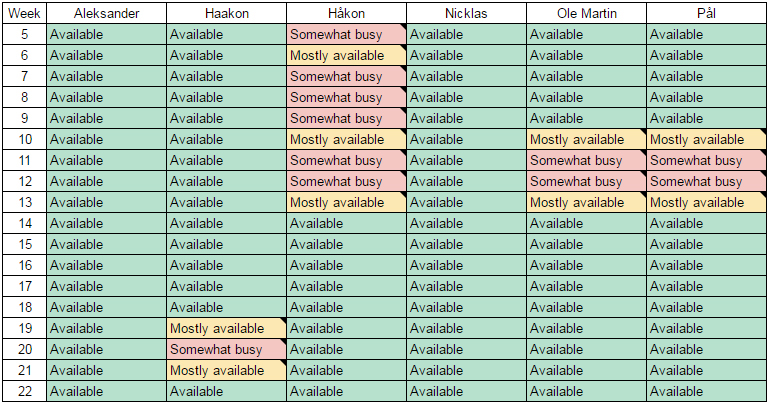
\includegraphics[width=\textwidth]{tables/planning/whereAreYou}
    \caption{Planned absence}
    \label{plannedAbsence}
\end{figure}


\section{Time frame}

\if  %% If False starts here #####################
\todo[inline]{ What to include: (Btw no clue how to structure this. Timeline, table, list, idk?)
\\ {[}Prio: Low{]} }
\begin{itemize}
    \item Feb 12. Preliminary report
    \item Feb 25. VERY early demo. Just thoughts and drawings
    \item March 7. Deadline for content:editor, auth and communication
    \item March 7. First working demo for client
    \item March 18. Midterm report
    \item March 31. Deadline for Search:back-end
    \item April 11. Deadline for Content:publication
    \item April 25. Deadline for Content:datasets and Content:site-administration
    \item May 1. Deadline for deploying the system
    \item May 31. Deadline final report. 
\end{itemize}
\fi   %% If False ends here #######################
Group members were expected to each spend roughly 20 hours per week on the project, as it is a 15 credits course.
This resulted in 120 work hours per week at the teams disposal. This was originally 140 hours, though a group member left the team and course early on. Despite this, it was still planned to have 3 teams each working on different tasks throughout most of the project. For some tasks this partitioning turned out to be too small or too big. In those cases, the relevant teams were adjusted accordingly. 

Figure \ref{fig:deadlines} shows a planned timeline for working on the various tasks. 

The deployment deadline was set to 1st of May. This was decided primarily to leave May for writing the report and documentation. It also left sufficient time in case of underestimated time required for development tasks.

Figure \ref{fig:deadlines} shows when to implement each service and which are being developed in parallel. Lines 1, 4, and 8 represent report deadlines, lines 2, 3, 6, 7, and 9 represent development deadlines and demonstrations of the system, and line 5 represents the Easter holiday. It is due to its span over the Easter that the search service task is as long as it is.

\begin{figure}[H]
    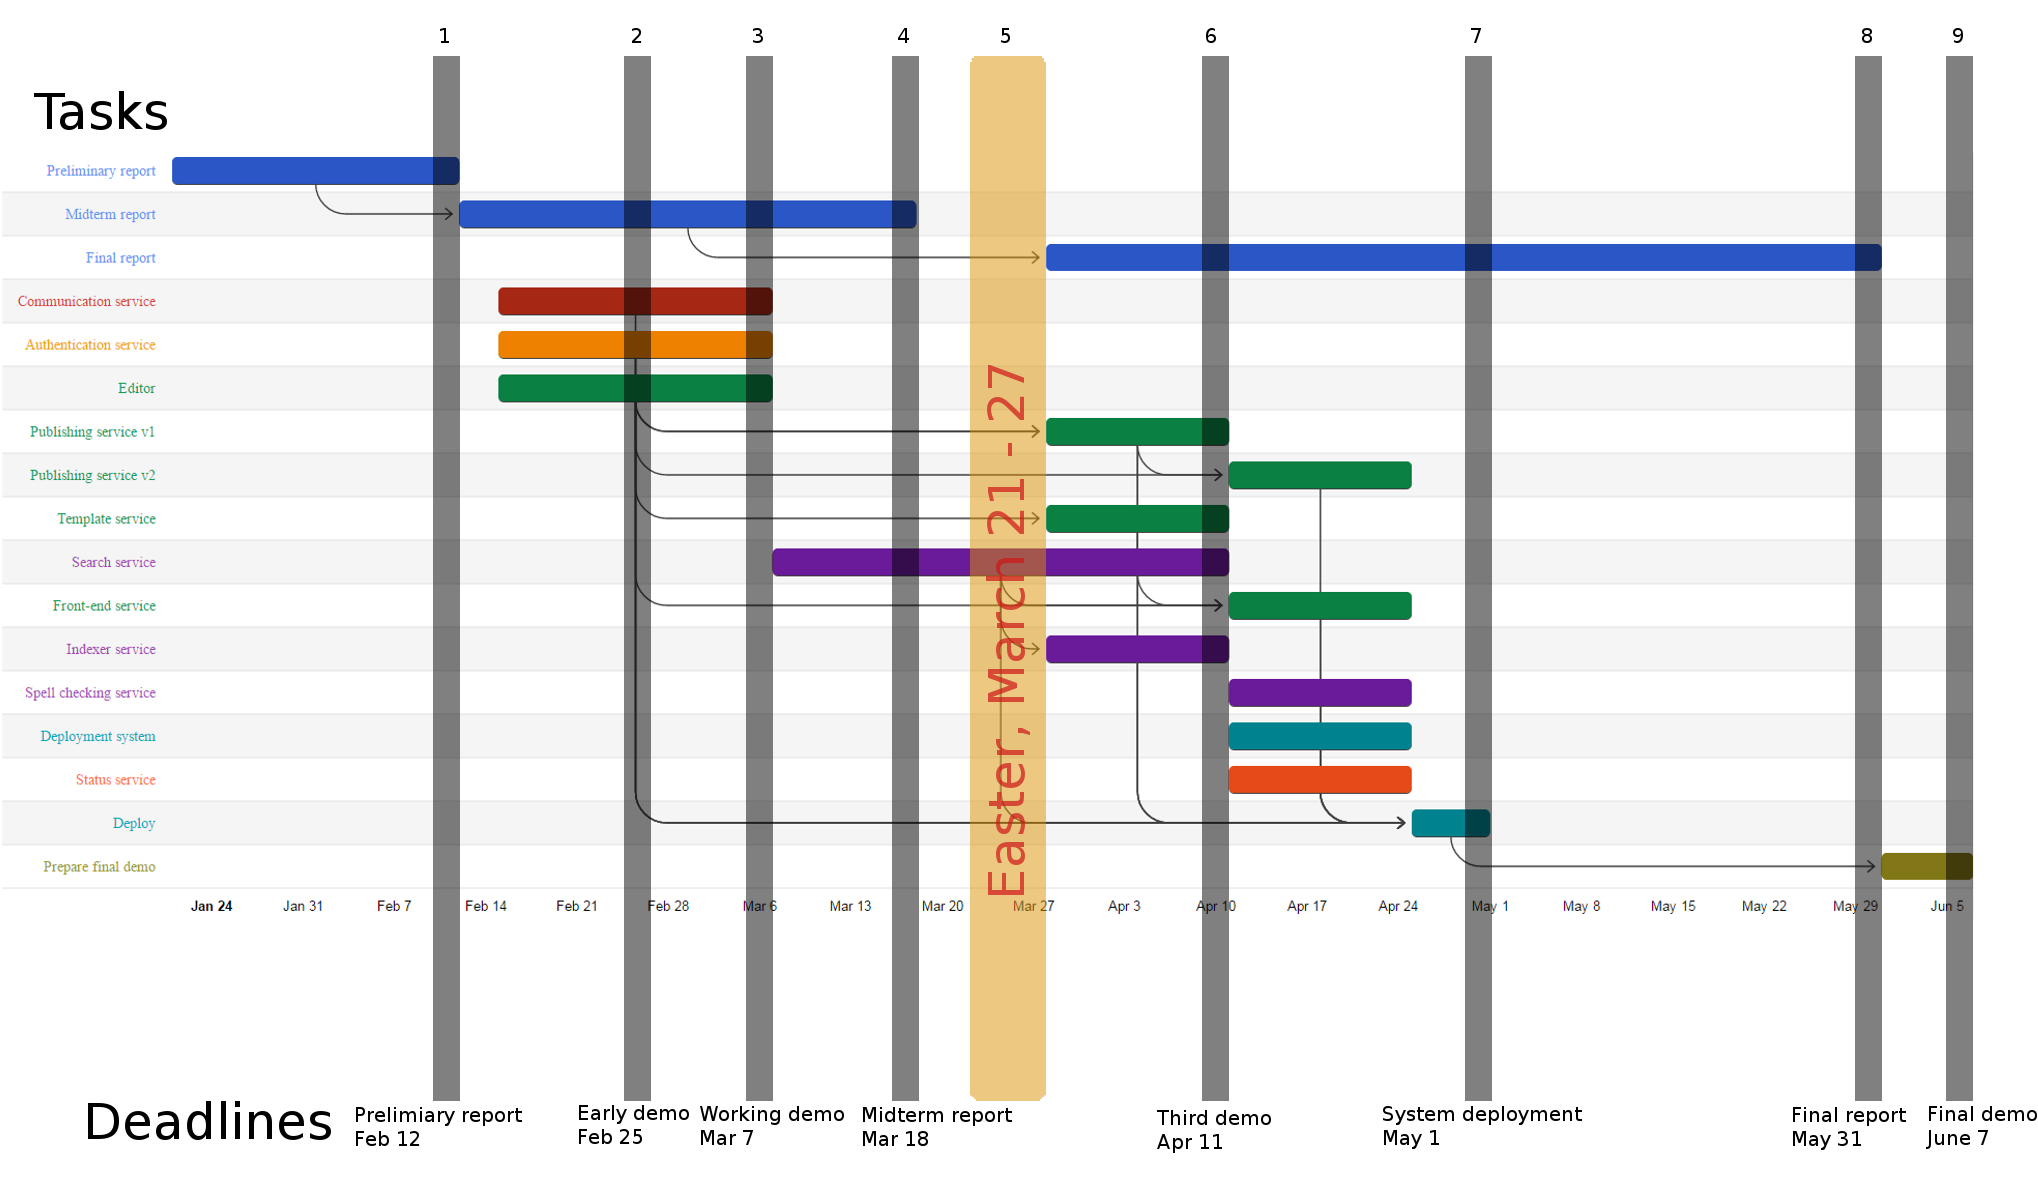
\includegraphics[width=\textwidth]{fig/plan}
    \caption{Activity plan with tasks and deadlines. Arrows indicates dependencies.}
    \label{fig:deadlines}
\end{figure}

\section{Estimation}

With a lot of focus on researching and exploring advantages, problems, and best practices -- estimating each task down to hours was both unpractical and infeasible. Some attempts towards estimating tasks in hours were made early in the project, though was quickly abandoned and story points were to a degree used instead \citep{storyPoints}. This allows for a more abstract estimate, while not committing to a fixed number of hours. In practice, the story points represented days until launch of the service, one day being about eight work hours. This type of measurement better handles all the uncertainties related to the research needed for each service. 

\section{The team}
During the first meeting, all the team members filled out a form with past experiences and language/technology familiarities. This was meant to be an aid for how to pick the members for the sub teams for the different microservices. The results from the meeting are displayed in table \ref{table:theTeam}. 

\begin{table}[H]
    \caption{The team, knowledge mapping}
    \centering
    %\begin{tabular}{| l | p{5cm} | p{5cm} | l }
    \begin{tabular}{|l|p{5cm}|p{5cm}<{\raggedright}|}
    \hline
    \textbf{Name} & 
    \textbf{Languages/technologies} & 
    \textbf{Experiences} 
    \\ \hline
    
    Aleksander Hansen & 
    Python, Java, C\#, C++, HTML, JS, LaTeX, MySQL, git & 
    IT1901
    \\ \hline
     
    Haakon Johansen Jonsson &
    Python, C/C++, Java, Scala, LaTex,  MySQL, Android, git & 
    Misc. small android projects, IT1901 
    \\ \hline
    
    Håkon Larsen Solbjørg & 
    Python {[Django]}, git, Java, HTML, JS, CSS, REST, LaTeX, UNIX, CI, Testing &
    dotkom, the startup Islero, IT1901
    \\ \hline
    
    Nicklas Nilsen & 
    Python, SQL, Fortran, LaTeX, git, UNIX & 
    IT1901 
    \\ \hline
    
    Ole Martin Knurvik & 
    Python, CSS, HTML, JS, Java {[Android]}, LaTeX, C\#, git & 
    Design and \acrshort{ui}, IT1901
    \\ \hline
    
    Pål Karlsrud & 
    Python {[Django, Flask]}, Java, C, Perl, Postgres, MySQL, UNIX, Apache, Shell, git, HTML, JS, CSS & 
    IT-Komiteen at Samfundet, IT1901
    \\ \hline
    \end{tabular}
    \label{table:theTeam}
\end{table}

\section{Team organisation}

The internal teams were assigned and reassigned based on the current requirements and technologies used, so having strictly defined roles throughout the project would have been cumbersome. Although some overarching responsibilities were assigned to some team members, to ease communications and knowing who to talk to regarding e.g.\ service hosting and operations during testing.

\subsection{Roles}
  
\paragraph{Group Leader} Ole Martin Knurvik\newline
The group leader took care of organisational tasks and delegated work to the other group members. Examples of tasks are booking meeting rooms, communicating with the customer and course staff, et cetera.
  
\paragraph{CTO} Håkon Larsen Solbjørg\newline
The \acrlong{cto} is a role which functions as an advisor. This can be useful when starting developing a feature, for example suggesting a programming language, framework, or library to use, or a sparring partner on how to implement a given functionality.


\subsection{Responsibilities}

\paragraph{UI and UX} Ole Martin Knurvik\newline
Has the executive role of design (\acrshort{ui} and \acrshort{ux}) for the front-end service(s) of the system. This covers following a graphic profile, making sure the design is clean, and that the system is usable from a usability perspective. This role originally included responsibility for usability testing and such, but was omitted seeing as this is not important for an architecture demonstration.

\paragraph{Deployment server(s) (production)} Pål Karlsrud\newline
Has the executive responsibility of managing the deployment server(s) that are used in a production environment.

% hihi, tusen takk! :D
% Ikke enda dessverre :p Drar dit straks! Yaaay! Masse flott lagg! Gleder meg masse. 
% Ohhhh! Det er sweet! Det kan egentlig hjelpe ganske mye :D

% HEI PÅL :D
% \paragraph{Gratulerer med dagen i går!} :D
% Er du på toget? TUUT TUUUUUT
% :(
% :'(((
% Sharelatex på NSB <33 blir sikkert bra. Websockets over treg 3G. 3ge? EHHEHEHEHEHHEH E HEHHEHEEH 
% Vi kan synce sharelatex mot github nå btw

% TakK!
% Vil du være med`?

% Det hadde vært litt dumt å bruke "chat" funksjonen i ShareLatex egentlig
% Det her er jo mye bedre
% Kan se alle typoene til folk underveis :D
% hahahah, en halv kek
%kek
% nice chat
%jeg er på vei nedover. skal prøve å rename sprintene 

% Bra vi hadde denne chatten i mellom to subparagraphs da, og ikke mellom den siste 
% paragrafen og neste section ,_,

% x)

% LA STÅ ^

\paragraph{Staging server(s) (development)} Pål Karlsrud and Håkon Larsen Solbjørg\newline
Has the executive responsibility of managing the staging server(s) that are used in a development environment.


\section{Software development process}
\label{section:devProcess}
The overarching guideline of the project was to explore and demonstrate the microservice architecture, rather than an implementation of the product itself. 
A consequence of this was that Scrum and Kanban would be difficult to strictly follow, as many of the elements from these methodologies would have seemed like wasted work. This includes elements like Scrum's product backlog, and Kanban's \acrshort{wip} limits. Initially Scrum was considered to be used as the main development process, but it was abandoned in the early phases of the project.
With a lot of time dedicated to reading up on microservices, methods, and technologies -- following a spiral model was more natural. 
A spiral model enables using part of the planning phase to do research, and iteratively determine the objectives and what functionality to implement \citep{sprialModel}.

This is not to say no elements from other methodologies were used. Daily stand-up meetings were used to keep everyone up to date on how the others were doing, allowing them to come with suggestions and feedback when needed. The objectives of each iteration could also be compared to the sprint backlog in Scrum, or To Do in Kanban. 


As shown in figure \ref{devMeth}, there are four main phases of each iteration. Each iteration started with research, as gathering knowledge about best practices, advantages, disadvantages, and customer preferences was essential in determining the next set of objectives -- in this case which functionalities to implement -- to best demonstrate microservices.

In step two of the iteration, determining the objectives, the client was often included and encouraged to come with feedback based on ideas and thoughts derived from the research. Once the objectives were established, the risks needed to be mapped out and resolved. In the fourth and final step, development and testing, the objectives were naturally implemented and tested before deployment. Due to the small size of each service this was either done alone or with a partner. In this part, techniques like pair programming or Kanban were options for use. This decision was left up to each team depending on what they felt more comfortable with. 


\begin{figure}[H]
    \centering
     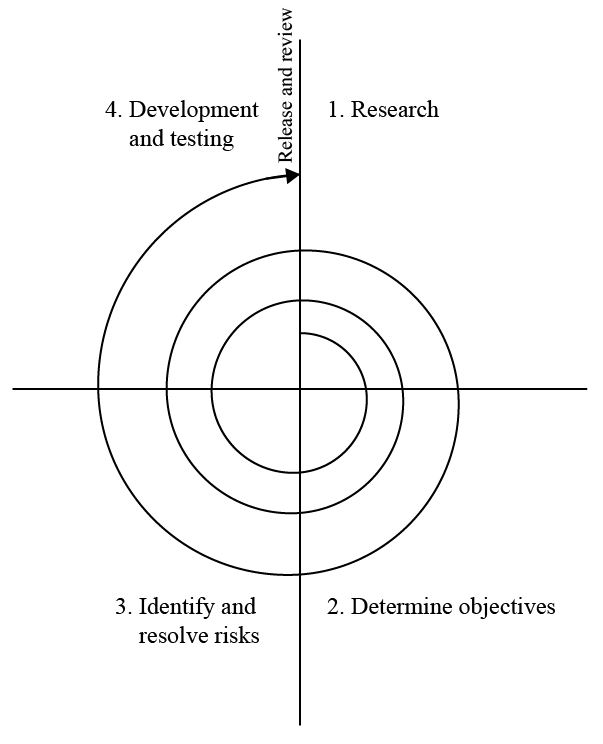
\includegraphics[scale=0.6]{fig/project_management/devMeth}
    \caption{Development method}
    \label{devMeth}
\end{figure}


\section{Iterations}
The length of each iteration has been a bit fluid and varied from one to three weeks. This due to the huge differences in size and uncertainty of each service implementation. Seeing as the team was split into groups which did not depend on each other, apart from the deadlines and deliveries, there was no reason why each group should be locked to the same length for each iteration. 

\subsection{Iteration 1}
\textbf{21st of February -- 7th of March} \\
\noindent During the first iteration, the focus was on three parts of the system: the editor, the authentication service, and the communication service.

The group was divided as follows:

\begin{flushleft}
\textbf{Editor}
\begin{itemize}
\itemsep -0.5em
  \item Haakon Johansen Jonsson
  \item Ole Martin Knurvik
\end{itemize}

\textbf{Authentication}
\begin{itemize}
\itemsep -0.5em
  \item Håkon Larsen Solbjørg
  \item Nicklas Grimstad Nilsen
\end{itemize}


\textbf{Communication}
\begin{itemize}
\itemsep -0.5em
  \item Pål Karlsrud
  \item Aleksander Hansen
\end{itemize}

\end{flushleft}

The goal of the iteration was to get a working prototype up and running for a demonstration with the customer the 7th of March.
This prototype was to consist of an editor, which was to communicate with the authentication service. This meant that a user should be able to log in and then use the editor. The user stories that cover this functionality is shown in table \ref{tab:iter1_stories}.

\begin{table}[H]
   \caption{User stories for iteration 1 }
   \centering
   \label{tab:iter1_stories}
   \begin{tabular}{|p{1.3cm}|p{6cm}|p{3cm}|p{2.5cm}|}\hline%
        ID & Description & Service & Story points\\\hline\hline
        
        CF-1 & As a user, I should be able to create articles using a \acrshort{wysiwyg} editor & Front-end & 8 \\ \hline
        CF-2 & As a user, I should be able to add and adjust images & Front-end & 3 \\ \hline
        CF-3 & As a user, I should be able to add videos to articles & Front-end & 3 \\ \hline
        CF-4 & As a user, I should be able to add links to other articles and to web pages & Front-end & 2 \\ \hline
		A-1 & As a user, I want to be able to log in & Auth & 8 \\ \hline
        A-4 & The system should allow for different access levels & Auth & 8 \\ \hline
        COM-1 & The services should be able to communicate with each other & Communication & 13 \\ \hline
        COM-2 & The services should be able to easily query for the \acrshort{ip} address of a given service & Communication & 3 \\ \hline
    \end{tabular}
\end{table}

Most of the iteration was spent on learning and choosing which technologies to use for the various services. This took a lot more time than originally anticipated, as the team had little experience with most of the technologies that were planned for use. This motivated the switch from Scrum to the spiral model.

Combining the services proved to be harder than expected.
While all the services worked by themselves at the end of the iteration, communication between the editor and the authentication service was not ready for the demonstration.

During the course of the iteration it was decided, in agreement with the customer, that a distributed communication system would be used. A \acrshort{wysiwyg}-type editor was chosen, and templates were to be fully editable. ``Embedded code'' was interpreted to mean embedded objects like video.
The requirements as they were before any changes were made is found in appendix \ref{requirements}.

\subsection{Iteration 2}
\textbf{28th of March -- 11th of April} \\
\noindent Between the 7th and 28th of March, only the search service was in development; the next proper iteration did not start before the 28th of March. This was due to Easter, having to write on the report, and a large part of the group being unavailable.

The second iteration focused on the first publishing service, the template service, the search service, and the index service.

The group was divided as follows:

\begin{flushleft}
\textbf{Publishing service}
\begin{itemize}
\itemsep -0.5em
  \item Haakon Johansen Jonsson
  \item Ole Martin Knurvik
\end{itemize}

\textbf{Template service}
\begin{itemize}
\itemsep -0.5em
  \item Pål Karlsrud
  \item Håkon Larsen Solbjørg
\end{itemize}


\textbf{search and indexer service}
\begin{itemize}
\itemsep -0.5em
  \item Nicklas Grimstad Nilsen
  \item Aleksander Hansen
\end{itemize}

\end{flushleft}

The goal of this iteration was to create an improved prototype, capable of demonstrating publishing and viewing of articles, searching, and loading templates. The user stories that cover the functionality in this iteration is shown in table \ref{tab:iter2_stories}.

\begin{table}[H]
   \caption{User stories for iteration 2 }
   \centering
   \label{tab:iter2_stories}
   \begin{tabular}{|p{1.3cm}|p{6cm}|p{3cm}|p{2.5cm}|}\hline%
        ID & Description & Service & Story points\\\hline\hline
        
        CF-5 & As a user, I should be able to view articles in an appropriate \acrshort{ui} & Front-end & 3 \\ \hline
        CT-1 & As a user, I should be able to choose a template for the article & Template & 13 \\ \hline
        CP-1 & As a user, I should be able to publish created articles & Publishing & 8 \\ \hline
        CP-2 & As a user, I should be able to edit metadata (tags and descriptions) of documents & Publishing & 2 \\ \hline
        SE-1 & As a user, I should be able to quickly search for documents & Search & 13 \\ \hline
    \end{tabular}
\end{table}

The improved prototype did have the features that were planned to be implemented in this iteration. The template and search services were not connected to the front-end, and had to be demonstrated by themselves. The publishing service however could demonstrate communication between services.

The original plan was to have every microservice supply their own user interface, and have the client-side load them individually
During the iteration it was decided that there would be a separate front-end service to deal with the user interface, because communication within the client-side of the project turned out to be really difficult. After the demonstration for the customer, an additional requirement -- having two implementations of the publishing service -- was added by request from the customer. It was also decided that features like calendar information, attachments, and support for different file types in the search service, were not important to the goal of the project, so the related requirements were removed.
% !TEX encoding = UTF-8 Unicode
% !TEX root = thesis.tex
% !TEX spellcheck = en-US
%%=========================================

\chapter{Alternative solutions}
\label{chapterAlternativeSolutions}

Following the microservice architecture with loosely coupled services, there are unbounded options and combinations of solutions for the frameworks alone. Many of the technologies chosen for the final solution were based on previous experience and knowledge, and some on their compatibilities with other solutions. This chapter discusses some of the choices that were made and alternatives that were considered.

%%=========================================
\section{Technologies}
The customer expressed a preference for microservices being implemented using a variety of technologies, so that the modularity- and separability benefits of microservices would become more apparent. Beyond that, the customer had no preferences for any specific technologies. The back-end of the search microservice was created in Python, because of familiarity with the language, as well as Python having a sizable set of libraries with the required functionalities. Python was not a necessity, however -- the team also had familiarity with Java and appropriate Java libraries -- so Java was an option as well.

Searching and indexing was implemented as two separate services. 
The main purpose of this decision was to further demonstrate the modularity of microservices; it would however be possible to replace the two services with a new conjoined service which provided both searching and indexing. An example of an alternative solution would be to use Apache Solr, which provides a superset of the functionality implemented by the current solution \citep{solr}.

Similar technology decisions were applicable for the other microservices as well, enabling a mixed composition of technologies to showcase the large degree of decoupling microservices posit.

\subsection{Deployment alternatives}
How the different services are deployed is especially important when working with microservices, as one of the goals with microservices is for it to be easy to add or remove instances of a service. The following alternatives for deployment of services were considered: using a single server for all services, creating a \acrshort{vm} for each service, and creating a Docker container for each service.

At first running all the services on the same server was considered. The problem with this is that the services would have been harder to distinguish, as they may run several similar processes \citep{dockerDzone}. Another problem is that this would make it relatively hard to scale to multiple servers, since all servers would need to run all services.

Running all the services on the same server would also provide very little isolation between the services. Lack of isolation might cause problems when using microservices, as it is common to use many different technologies which provide some of the same functions, and this might cause the technologies to interfere with each other.

Using \acrshort{vm}s for each of the services solves many of the problems above. A disadvantage with \acrshort{vm}s is that they have high overhead, as they usually run a full operating system. \acrshort{vm}s do however provide more isolation than with Docker containers or running the services directly on a server \citep{devopsDockerVSVM}, though at the cost of more overhead.

Not needing quite the isolation that \acrshort{vm}s provide, Docker containers was chosen for deployment. While being more lightweight than \acrshort{vm}s, Docker also makes it easy to deploy custom, sandboxed, self-contained environments for each of the services, which means that a specific microservice can be started and stopped or replaced, without affecting other services \citep{devopsDockerVSVM}.

The Docker containers are run on a Debian server. Debian was chosen for its stability and high level of documentation. Windows, Ubuntu, or Fedora were options as well, but Debian has more server related documentation, and is more minimalistic than Ubuntu \citep{whyDebian}. Each Docker container uses Alpine Linux, as this provides a minimal operating system while still providing all the services and packages required \citep{alpineLinux}.

\subsection{API structure}
Multiple services needing to communicate introduced the need for well-defined \acrshort{api}s. A service accesses the functionality of a target service through the target's \acrshort{api}. For instance, a service responsible for hosting content might require clients to have specific permissions, necessitating a service for authenticating users and proving the authentication state of users.

\acrshort{rest} \acrshort{api}s exposing \acrshort{json} data was chosen as the underlying interface technology, and the \acrshort{dry}-principle for communication between the various services, although \acrshort{soap} and \acrshort{wsdl} are viable alternatives for defining and exposing the functionalities of the various services through \acrshort{xml}-formatted data rather than \acrshort{json}.


\subsection{Service-to-service communication alternatives}\label{subsec:alternative_arch}
The way the microservices communicate is a very important part of the microservice architecture, as it largely determines how loosely coupled the services will be \citep{pwcMicroservices}.

The following three communication architectures were considered: having the services communicate directly, using a message-broker, and using a fully distributed architecture.
Tables \ref{table:pros_cons_gateway}, \ref{table:pros_cons_broker}, and \ref{table:pros_cons_distr} summarise the pros and cons of these architectures.

\begin{table}[H]
\caption{Pros and cons of direct communication} 
\begin{tabularx}{\linewidth}{>{\parskip1ex}X@{\kern4\tabcolsep}>{\parskip1ex}X}
\toprule
\hfil\bfseries Pros & \hfil\bfseries Cons\\
\cmidrule(r{3\tabcolsep}){1-1}\cmidrule(l{-\tabcolsep}){2-2}

%% PROS
Simple\par
Easy to scale\par
Easy to monitor\par

&

%% CONS
Potential single point of failure\par
Requires some form of service discovery and registry\par

\end{tabularx}
\label{table:pros_cons_gateway}
\end{table}

Direct communication (illustrated in figure \ref{fig:alternativeDirectComm}) was considered early on. In the illustration, service B and C wishes to communicate with service A. For this to be possible, service B and C each need the \acrshort{ip} address of service A -- so to enable the service-to-service transmission of content.

\begin{figure}[H]
    \centering
    \scalebox{1.4}{\tikzstyle{service}=[draw, text width=5em, 
    text centered, minimum height=2.5em,
    fill=blue!20]

\begin{tikzpicture}    
    \node[service] (A) {Service A};
    \node[service] (B) [right=2cm of A] {Service B};
    \coordinate (mid) at ($(A)!0.5!(B)$);
    \node[service] (C) [below=2cm of mid] {Service C};
    

    \draw[<->,thick] (A) -- (B);
    \draw[<->,thick] (A) -- (C);
\end{tikzpicture}
}
    \caption{Example of communication using direct communication.}
    \label{fig:alternativeDirectComm}
\end{figure}

The plan was to use an automated service discovery program called Registrator \citep{registrator}, along with the key/value store features of Consul \citep{consulMicroservice}. The advantage of this approach would be that to obtain the \acrshort{ip} address of a service, a service need only know how to query Consul. The role of Registrator would have been to automatically register services using Consul.

However, Registrator turned out to not be as suitable as it at first seemed, since it lacked proper support for versioning of \acrshort{api}s. 
Registrator also lacked features for making services available only after the service had actually started up -- this is important, as a service might use some time to start, during which it might not be ready to accept requests.

In order to find a solution which could easily be modified to fit the needs of the system, a message-broker architecture was considered. This would solve the notification problem by having each service register itself, and periodically send heartbeat messages to the broker, to signal that the service is still online.
A message broker architecture would also remove the need for direct communication, and instead allow the services to communicate using channels provided by the broker \citep{nginxMicroservicesMessageBroker}.

\begin{table}[H]
\caption{Pros and cons of message brokers}
\begin{tabularx}{\linewidth}{>{\parskip1ex}X@{\kern4\tabcolsep}>{\parskip1ex}X}
\toprule
\hfil\bfseries Pros
&
\hfil\bfseries Cons\\
\cmidrule(r{3\tabcolsep}){1-1}\cmidrule(l{-\tabcolsep}){2-2}

%% PROS
Fast\par
The clients only need to know about the relevant channels\par
Scales well with multiple services\par

&

%% CONS
Potentially single point of failure\par
Hard to change message format\par
Must have relevant bindings for language used in microservice\par
\\\\\end{tabularx}
\label{table:pros_cons_broker}
\end{table}

Figure \ref{fig:alternativeMessageBroker} illustrates how the services would communicate with each when using a message broker. Using the message broker architecture, service B and C would send a message to the broker in order to communicate with A. The broker would function similarly to a router, since it routes messages between services.

\begin{figure}[H]
    \centering
     %\includegraphics[scale=0.7]{fig/alternative-solutions/message-broker}
    \scalebox{1.0}{\tikzstyle{service}=[draw, text width=5em, 
    text centered, minimum height=2.5em,
    fill=blue!20]

\tikzstyle{broker}=[draw, text width=4em, 
    text centered, minimum height=2em,diamond,
    fill=black!40]
\begin{tikzpicture}    
    
    \node[broker] (broker) {Broker};
    \node[service] (A) [below=of broker] {Service A};
    \node[service] (B) [above=of broker] {Service B};
    \node[service] (C) [right=of broker] {Service C};
    

    \draw[<->,thick] (broker) -- (A);
    \draw[<->,thick] (broker) -- (B);
    \draw[<->,thick] (broker) -- (C);
\end{tikzpicture}
}
    \caption{Illustration of communication using a message broker.}
    \label{fig:alternativeMessageBroker}
\end{figure}

For larger networking loads, communication using message brokers tends to be easier to scale than direct communication, by enabling asynchronous communication. This results in endpoints being able to offload the responsibility of transporting messages \citep{nginxMicroservicesMessageBroker}.

This did however require writing a solution from scratch, which proved more difficult than it first seemed, particularly because large parts of the message handling had to be written from the bottom-up, 
and none of the frameworks that were looked into, such as ZeroMQ and RabbitMQ, would allow easily creating the messaging pattern shown in figure \ref{fig:alternativeMessageBroker}.

Further consideration resulted in an architecture using \acrshort{dht} to store the \acrshort{ip} addresses for each service. This is illustrated in figure \ref{fig:alternativeDHT}. In this architecture, each of the nodes in the \acrshort{dht} collectively store the \acrshort{ip} addresses associated with each service, and when a service wishes to connect to another service, it need only query the \acrshort{dht} to obtain an \acrshort{ip} address.

\begin{table}[H]
\caption{Pros and cons of a fully distributed system} 
\begin{tabularx}{\linewidth}{>{\parskip1ex}X@{\kern4\tabcolsep}>{\parskip1ex}X}
\toprule
\hfil\bfseries Pros & \hfil\bfseries Cons\\
\cmidrule(r{3\tabcolsep}){1-1}\cmidrule(l{-\tabcolsep}){2-2}

%% PROS
No single point of failure\par
Relatively easy to query\par

&

%% CONS
Complex\par 
Takes some time before a node is marked as dead\par
Makes changes to the communication system harder to implement.
\\\end{tabularx}
\label{table:pros_cons_distr}
\end{table}

This alternative eliminates the single point of failure, and each of the nodes used to store information in the network can easily be replaced without bringing down the entire network.
Cursory research did not result in finding any other microservice projects having used this approach, making it an interesting solution to explore.

Figure \ref{fig:alternativeDHT} illustrates how the \acrshort{dht} architecture works. Service B and C first need to request the \acrshort{ip} address to an instance of service A, and then communicate directly with service A using the received \acrshort{ip} address.

\begin{figure}[H]
    \centering
    \scalebox{1.1}{\tikzstyle{service}=[draw, text width=5em,
    text centered, minimum height=2.5em,
    fill=blue!20]
\tikzstyle{dht}=[draw, text width=2em,
    text centered, minimum height=2.5em,
    fill=black!10,cloud]

\begin{tikzpicture}
    \small;
    \node[dht] (dht) {DHT};
    \node[service] (B) [left=4cm of dht] {Service B};
    \node[service] (C) [right=4cm of dht] {Service C};
    \node[draw=none] (reg) at($(dht)!0.4!(B)$) {};
    \node[service] (A) [below=2cm of reg] {Service A};

    \draw[<->,thick,shorten >=0.3mm] (B) -- (dht) node[pos=0.5,above] {Get IP to service A};
    \draw[<->,thick,shorten >=0.3mm] (C) -- (dht) node[pos=0.5,above] {Get IP to service A};
    \draw[<->,thick] (A) -- (dht) node[pos=0.8,left] {Register as service A};
    \draw[<->,thick] (B) -- (A.north west) node[pos=0.5,below left] {Communication};
    \draw[<->,thick] (C) -- (A.north east) node[pos=0.5,below right] {Communication};

\end{tikzpicture}}
    \caption{Communication between services using the \acrshort{dht} architecture.}
    \label{fig:alternativeDHT}
\end{figure}


\section{Development method alternatives}
A spiral model based development method was chosen (as explained in section \ref{section:devProcess}). Alternatives like Scrum, Kanban and Waterfall were discussed, though all fell a bit short. The requirements were likely to change, and services were likely be added or removed, so following a waterfall method was considered unpractical. This is because Waterfall requires a lot of planning early in the project, when in the case of this project all the information needed was not yet available.

A solution implementing Kanban or Scrum could have worked, but seeing as how much the requirements and functionality was changing, having a strict backlog and organising it would require much effort, while giving few benefits \citep{scrumVideo}. Also many of the team members were inexperienced in using agile development or the artifacts they come with.

% !TEX encoding = UTF-8 Unicode
%!TEX root = thesis.tex
% !TEX spellcheck = en-US
%%=========================================
\chapter{Tools and technologies}
\label{chapterToolsTech}\label{chap:tools_technologies}

This chapter describes the tools and technologies used. This includes development tools and frameworks used, like version control systems, programming languages, and third party frameworks and libraries.


%%=========================================
\section{Development tools}

\subsection{Git}
\label{subsection:git}
Git was chosen for version control, with GitHub as the repository hosting service. Git was chosen as it makes it easy to manage code, and every team member had experience using it.

\subsection{Go}
The Go programming language was used for the microservice which hosts templates. Go was primarily chosen because it makes concurrent operations easy, which makes it simpler to make a high performance service \citep{whyGo}. 

\subsection{Python}
Python was used for most of the microservices, as it was the language most of the group members was experienced in. One of the main advantages with Python is that it enables quick prototyping, and at the same time tends to result in manageable and modular code. Several different Python frameworks were used for the microservices. 

\paragraph{Django} web framework was used for the front-end and one of the publishing services, since it is well established with good documentation, a lot of supported packages and is actively developed. Also, some team members already had experience with it, and it seemed fairly easy to learn for those familiar with Python.

\paragraph{Twisted} is an event-driven asynchronous networking engine for Python. Twisted was chosen for several of the services because it is quick to set up and configure, without a lot of web-server boilerplate \citep{twisted}.

\paragraph{Entangled} is a \acrshort{dht} and tuple space based on Kademlia written in Python \citep{entangled}. The project was forked from its GitHub repository and used as a starting point for the communication back-end.

\subsection{JavaScript}
JavaScript was used for client side scripting and for the server side of one of the publishing services.

\paragraph{Summernote} is a JavaScript library for creating simple \acrshort{wysiwyg} editors \citep{summernote}. It was chosen as the basis for the editor because it is not very complex, it creates a simple user interface, it is fairly easy to modify if needed, and it still covers our requirements.

One of the publishing services is written in JavaScript to demonstrate that the microservices can be written in different languages and still be compatible and interchangeable with each other. JavaScript was chosen to achieve diversity without using a great deal of unfamiliar languages.

\paragraph{Node.js} was used as the JavaScript runtime environment with the Express.js web framework. This was because they seemed to be the most established and documented tools for their respective tasks.

\subsection{MongoDB}
MongoDB is a document database. It was chosen for the publishing and templates services because their task is primarily to store and retrieve article and template documents, which is what a document-oriented database like MongoDB is designed for \citep{MongoDB}. MongoDB is also easy to work with, since it stores documents in a \acrshort{json}-like format, and data is usually formatted as \acrshort{json} when it is transferred between microservices. This was also a good opportunity for some group members to learn about NoSQL databases.

\subsection{PostgreSQL}
PostgreSQL is an open source database system. It was chosen for the indexing service. PostgreSQL was chosen as it provides a combination of stability and performance \citep{whyPostgres}. 

\section{Deployment tools}
The following subsections describe the tools that are in use to facilitate an easier deployment phase. All the microservices run containerised behind a reverse \acrshort{http} proxy, and all logs are shipped to a central repository. Due to the \acrshort{devops} methodology, all services are continuously deployed, and therefore continuous integration tools were required.

\subsection{Docker} \label{subsec:docker}
Docker is a tool that spawns an application in a containerised environment. It behaves much like a virtual machine, but it shares several of the base components with the host.  By doing so, Docker provides isolation between different containers, while remaining lightweight. It has a simple command line for managing containers, which makes it very easy add or remove new services, and add new instances of existing services.

Virtual machines abstract away the hardware components of the host machine and emulate their own. This makes it possible to run the same system almost anywhere, with the same components -- even though the host machine is different.

\subsection{Docker Compose}
Docker Compose is a command-line interface for managing multi-container Docker applications, and makes it easy to scale and upgrade the system by providing commands for these specific actions \citep{dockerCompose}.

\subsection{Nginx}
Nginx is a an open source web server. This provides a common interface for load balancing and routing from the Internet to the different microservices.


\subsection{Teamcity}\label{subsec:technologies-teamcity}
TeamCity is a \acrshort{ci} system. It is provided for free and runs tests for each service upon a version control check in, giving feedback on whether tests pass. \acrshort{ci} and testing is described in chapter \ref{chap:testing}.

\subsection{Jenkins}
Jenkins is a \acrshort{ci} system, which was used to automatically deploy the services. Jenkins was chosen as it provides several plug-ins for deploying Docker containers.

\subsection{Travis CI}\label{subsec:technologies-travis}
Travis is another \acrshort{ci} system. It is distributed and runs in the cloud rather than on premise, which allows for very simple test-running for small systems. Travis was chosen for the service used to serve templates, as the service was written in Go, which is incompatible with TeamCity, as well as requiring special accessories not integrated in TeamCity by default.

\subsection{Logstash}
Since every service is run in a containerised environment, an application to centralise the log files produced by each service was needed -- otherwise the container of each service would have to be accessed to obtain the log files. Logstash was used to solve this problem. Logstash is an application which makes it easy to centralise log files produced by multiple servers and make them accessible in a shared format \citep{logstash}.

\section{Testing} \label{section:tools_tech_testing}
For testing, the libraries associated with the specific programming languages was primarily used, as specialised libraries are more flexible than forcing all tests into a specific framework. When releasing new versions of the microservices, all the tests are run using a \acrshort{ci} system. This ensures that all tests pass before the new version is actually released. Read more about testing strategies in chapter \ref{chap:testing}.

\section{Project management tools}
Seeing as git was already being used for code, all the other documents could have been synced through it as well. However, for real-time collaboration on the same files, real-time editing tools like Google Drive and ShareLaTeX were used instead.

\paragraph{Google Drive} was used for all project related documents, such as plans, meeting summaries, and illustrations. Google Drive was chosen due to its real-time collaboration for creating and editing a wide variety of files, in addition to simply uploading and sharing most other file types.

The reason why Google Drive was chosen, is that it has excellent integration with the Google Docs system, which makes it easy to edit and create new documents.

\paragraph{ShareLaTeX} was used for easy collaboration when writing the report in LaTeX. It is also significantly more user friendly than the normal LaTeX toolchain, and allows collaborative real-time editing. The report could have been edited locally, and then synchronised using git via GitHub, but this would most likely cause many merge conflicts and would make it cumbersome to write the report. 

\section{Communication tools}
\label{sectionCommunicationTools}
The group members, the client, and the supervisor all had very different time schedules. This necessitated some sort of asynchronous online communication platform. 

\paragraph{E-Mail} was chosen as the main communication platform with both the client and the supervisor outside the meetings. E-mail enables participants to answer when they have time to spare, without having the expectation to always reply immediately that more instant messaging applications do. 

\paragraph{Slack} was chosen as the main communication tool within the group. Slack allows for creating chat groups for different topics (e.g. Report writing, testing, general). A plugin for slack called Geekbot was also used. Geekbot is a stand-up bot, which each day asks all members of the team what they achieved yesterday, what they plan on doing today and what (if anything) is impeding their progress \citep{geekbot}. This requires less commitment than physical stand-up meetings, and is especially helpful when the team is not able to meet on a daily basis. 
% !TEX encoding = UTF-8 Unicode
%!TEX root = thesis.tex
% !TEX spellcheck = en-US
%%=========================================
\chapter{Architecture}
\label{chapterArchitecture}

The architecture, and especially communication between services, is important when creating microservices, as this largely determines the maintainability, efficiency, and modularity of the system.
Choosing a suiting architecture is therefore very important.

\section{System architecture}
When building a microservice based system, it is important to consider the granularity of the services \citep{granularity}. A coarse grained interface was chosen, i.e. each service receives and sends \acrshort{json} structured information. The goal of each service is to have a well-defined function and that each microservice consists of components that are easy to reuse. By making each service have a well-defined function, a loose-coupling between the services can be maintained.

Without loose coupling, modifying a service often necessitates modifying all services that interacts with it. This can become a problem in monolithic and to an extent service-oriented architectures, because of their unclear guidelines for separating services \citep{ibmSoaDescription}.

This system consists of eight microservices. They are described in section \ref{sec:microservices}, and the architecture shown in figure \ref{fig:fullarkitektur}. One of the services has two implementations, in two different programming languages, in order to show how a service could easily be replaced in the microservice architecture. The status service is not shown in figure \ref{fig:fullarkitektur}, as it performs monitoring, and is not part of the \acrshort{cms} system.


\begin{figure}[H]
    \centering
     \includegraphics[scale=0.4]{fig/architecture/system-architecture}
    \caption{Connections between different microservices and other components.}
\end{figure}\label{fig:fullarkitektur}

\section{How the services communicate}
A \acrshort{dht} works by distributing the responsibility for maintaining the mapping from keys to values among the nodes in the network. As  mentioned in section \ref{subsec:alternative_arch}, this property is exploited to store the type of service and the \acrshort{ip} addresses associated with that type. This also automatically distributes the load among all nodes, and by doing so fulfils NFR-5.

The node is divided into two parts: one part for communicating with the other nodes in the network, and one part which exposes a \acrshort{rest} \acrshort{api} to the service, so that it can easily query the network for \acrshort{ip} addresses.

This removes the need for creating language specific bindings, and makes the node easier to test, as \acrshort{http} requests are sufficient to obtain data from a given node. Each service runs a node as a part of the microservice.

When a service $A$ wants to communicate with another service of type $B$, it begins by querying the node to obtain an \acrshort{ip} address to a node $C$ of type $B$. This allows service $A$ to communicate directly with $C$. If $A$ detects that $C$ does not respond, it simply removes $C$ from the list of available services. This flow is illustrated in figure \ref{fig:comm_example}
\begin{figure}[H]
    \centering
    \includegraphics[scale=0.30]{fig/architecture/communication-example}
    \caption{Flow of requests during a query.}\label{fig:comm_example}
\end{figure}

\section{The architecture of each microservice}\label{sec:microservices}

Originally there were five microservices related to the creation and publishing of content: editor, publishing, datasets, administration, and template service. These would form the core of the system. Figure \ref{fig:content_arch} shows an overview of their architecture.

It was however decided that the datasets and administration services would be unnecessary for the purpose of demonstrating the microservice architecture, so they were excluded.

It was also decided that having all the microservices supply their own front-end would be cumbersome and unnecessary, because many of them had very small or no front-end at all. So instead, all the front-ends were merged into a unified front-end service. The editor turned out to not need its own back-end at all, so it was entirely merged into the front-end service. An overview of the new content architecture is shown in \ref{fig:content_arch_new}.

\begin{figure}[H]
    \centering
    %\includegraphics[scale=0.20]{fig/architecture/content}
    \scalebox{0.8}{\pgfdeclarelayer{background}
\pgfdeclarelayer{foreground}
\pgfsetlayers{background,main,foreground}

\tikzstyle{object}=[draw, text width=5em, 
    text centered, minimum height=2.5em]

\tikzstyle{DB}=[draw, text width=2em, 
    text centered, minimum height=2em,circle]
%\tikzstyle{user}=[draw, text width=7em,
%    text centered, minimum height=2em,diamond]
\tikzstyle{user}=[draw=none]

\begin{tikzpicture}    
    \node[user] (admin) {Administrator};
    \node[object] (admin_front) [below=of admin] {Admin front-end};
    \node[object] (admin_back) [below=of admin_front] {Admin back-end};
    \node[DB] (admin_db) [left=of admin_back] {DB};

    \node[object] (publish_back) [right=2cm of admin_back] {Publisher back-end};
    \node[object] (publish_front) [above=of publish_back] {Publisher front-end};
    \node[DB] (publish_db) [below=of publish_back] {DB};

    \node[object] (editor_back) [right=2cm of publish_back] {Editor back-end};
    \node[object] (editor_front) [above=of editor_back] {Editor front-end};

    \node[object] (templates) [right=2cm of editor_back] {Templates};
    \node[DB] (templates_db) [right=of templates] {DB};

    \coordinate (mid) at ($(publish_front)!0.5!(editor_front)$);
    \node[user] (employee) [above=2cm of mid] {Employee};

    \node[object] (datasets_front) [right=1cm of employee] {Datasets front-end};
    \node[object] (datasets_back) [right=of datasets_front] {Datasets back-end};
    \node[DB] (datasets_db) [right=of datasets_back] {DB};


    \draw[<->,thick] (admin) -- (admin_front);
    \draw[<->,thick] (admin_front) -- (admin_back);
    \draw[<->,thick] (admin_back) -- (admin_db);
    \draw[<->,thick] (admin_back) -- (publish_back);
    \draw[<->,thick] (publish_back) -- (publish_db);
    \draw[<->,thick] (publish_back) -- (publish_front);
    \draw[<->,thick] (editor_back) -- (publish_back);
    \draw[<->,thick] (editor_back) -- (editor_front);
    \draw[<->,thick] (templates) -- (editor_back);
    \draw[<->,thick] (templates) -- (templates_db);
    \draw[<->,thick] (employee) -- (publish_front);
    \draw[<->,thick] (employee) -- (editor_front);
    \draw[<->,thick] (employee) -- (datasets_front);
    \draw[<->,thick] (datasets_front) -- (datasets_back);
    \draw[<->,thick] (datasets_back) -- (datasets_db);

    \def\FILL{blue!20}
    %\def\FILL{yellow!20}
    %\def\FILL{none}
    \begin{pgfonlayer}{background}
        \path (admin_front.north -| admin_db.west)+(-0.5,0.3) node (a) {};
        \path (admin_db.south -| admin_back.east)+(+0.3,-0.2) node (b) {};
        \path[fill=\FILL, 
            rounded corners, draw=black!50, dashed]
            (a) rectangle (b);


        \path (publish_front.north -| publish_front.west)+(-0.5,0.3) node (a) {};
        \path (publish_db.south -| publish_db.east)+(+0.8,-0.2) node (b) {};
        \path[fill=\FILL,
            rounded corners, draw=black!50, dashed]
            (a) rectangle (b);

        \path (editor_front.north -| editor_front.west)+(-0.5,0.3) node (a) {};
        \path (editor_back.south -| editor_back.east)+(+0.3,-0.2) node (b) {};
        \path[fill=\FILL, 
            rounded corners, draw=black!50, dashed]
            (a) rectangle (b);

        \path (templates.north -| templates.west)+(-0.5,0.3) node (a) {};
        \path (templates.south -| templates_db.east)+(+0.3,-0.2) node (b) {};
        \path[fill=\FILL, 
            rounded corners, draw=black!50, dashed]
            (a) rectangle (b);

        \path (datasets_front.north -| datasets_front.west)+(-0.5,0.3) node (a) {};
        \path (datasets_front.south -| datasets_db.east)+(+0.3,-0.2) node (b) {};
        \path[fill=\FILL, 
            rounded corners, draw=black!50, dashed]
            (a) rectangle (b);


    \end{pgfonlayer}
\end{tikzpicture}
}
    \caption{Overview of the original design of the content services.}\label{fig:content_arch}
\end{figure}

\begin{figure}[H]
    \centering
    \scalebox{0.8}{\pgfdeclarelayer{background}
\pgfdeclarelayer{foreground}
\pgfsetlayers{background,main,foreground}

\tikzstyle{object}=[draw, text width=5em, 
    text centered, minimum height=2.5em]

\tikzstyle{DB}=[draw, text width=2em, 
    text centered, minimum height=2em,circle]
%\tikzstyle{user}=[draw, text width=7em,
%    text centered, minimum height=2em,diamond]
\tikzstyle{user}=[draw=none]

\begin{tikzpicture}    
    %\node[user] (admin) {Administrator};
    %\node[object] (admin_front) [below=of admin] {Admin front-end};
    %\node[object] (admin_back) [below=of admin_front] {Admin back-end};
    %\node[DB] (admin_db) [left=of admin_back] {DB};

    %\node[object] (publish_back) [right=2cm of admin_back] {Publisher back-end};
    \node[object] (publish_back)  {Publisher back-end};
    %\node[object] (publish_front) [above=of publish_back] {Publisher front-end};
    \node[DB] (publish_db) [below=of publish_back] {DB};

    \node[object] (editor_back) [right=2cm of publish_back] {UI back-end};
    \node[object] (editor_front) [above=of editor_back] {UI front-end};

    \node[object] (templates) [right=2cm of editor_front] {Templates};
    \node[DB] (templates_db) [right=of templates] {DB};

    %\coordinate (mid) at ($(publish_front)!0.5!(editor_front)$);
    %\node[user] (employee) [above=2cm of mid] {Employee};
    \node[user] (employee) [above=of editor_front] {Employee};

    %\node[object] (datasets_front) [right=1cm of employee] {Datasets front-end};
    %\node[object] (datasets_back) [right=of datasets_front] {Datasets back-end};
    %\node[DB] (datasets_db) [right=of datasets_back] {DB};


    %\draw[<->,thick] (admin) -- (admin_front);
    %\draw[<->,thick] (admin_front) -- (admin_back);
    %\draw[<->,thick] (admin_back) -- (admin_db);
    %\draw[<->,thick] (admin_back) -- (publish_back);
    \draw[<->,thick] (publish_back) -- (publish_db);
    %\draw[<->,thick] (publish_back) -- (publish_front);
    \draw[<->,thick] (editor_back) -- (publish_back);
    \draw[<->,thick] (editor_back) -- (editor_front);
    \draw[<->,thick] (templates) -- (editor_front);
    %\draw[<->,thick] (templates) -- (publish_back);
    
    \draw[<->,thick] (templates) -- (templates_db);
    %\draw[<->,thick] (employee) -- (publish_front);
    \draw[<->,thick] (employee) -- (editor_front);
    %\draw[<->,thick] (employee) -- (datasets_front);
    %\draw[<->,thick] (datasets_front) -- (datasets_back);
    %\draw[<->,thick] (datasets_back) -- (datasets_db);

    \def\FILL{blue!20}
    %\def\FILL{yellow!20}
    %\def\FILL{none}
    \begin{pgfonlayer}{background}
        %\path (admin_front.north -| admin_db.west)+(-0.5,0.3) node (a) {};
        %\path (admin_db.south -| admin_back.east)+(+0.3,-0.2) node (b) {};
        %\path[fill=\FILL, 
        %    rounded corners, draw=black!50, dashed]
        %    (a) rectangle (b);


        %\path (publish_front.north -| publish_front.west)+(-0.5,0.3) node (a) {};
        \path (publish_back.north -| publish_back.west)+(-0.5,0.3) node (a) {};
        \path (publish_db.south -| publish_db.east)+(+0.8,-0.2) node (b) {};
        \path[fill=\FILL,
            rounded corners, draw=black!50, dashed]
            (a) rectangle (b);

        \path (editor_front.north -| editor_front.west)+(-0.5,0.3) node (a) {};
        \path (editor_back.south -| editor_back.east)+(+0.3,-0.2) node (b) {};
        \path[fill=\FILL, 
            rounded corners, draw=black!50, dashed]
            (a) rectangle (b);

        \path (templates.north -| templates.west)+(-0.5,0.3) node (a) {};
        \path (templates.south -| templates_db.east)+(+0.3,-0.2) node (b) {};
        \path[fill=\FILL, 
            rounded corners, draw=black!50, dashed]
            (a) rectangle (b);

        %\path (datasets_front.north -| datasets_front.west)+(-0.5,0.3) node (a) {};
        %\path (datasets_front.south -| datasets_db.east)+(+0.3,-0.2) node (b) {};
        %\path[fill=\FILL, 
        %    rounded corners, draw=black!50, dashed]
        %    (a) rectangle (b);


    \end{pgfonlayer}
\end{tikzpicture}
}
    \caption{Overview of the refactored design of the content services.}\label{fig:content_arch_new}
\end{figure}

The search microservice was also changed. Originally, it was supposed to be a single microservice -- but the team responsible for implementing it decided to split it into three microservices, as it would otherwise have to be larger than first anticipated.

\subsection{Front-end service}
The front-end of the project uses Django to render the pages according to templates. This service works by asking other services for content and displaying it to the user in its proper template. By having one service render all of the visible content, it is easy to change the overall look and feel without having to change more than one service. It also uses some JavaScript to implement Summernote as the \acrshort{wysiwyg} editor. 

\subsection{Publishing service}
The publishing service provides an \acrshort{http} \acrshort{api} to store and retrieve articles and information about articles, and to get a list of currently stored articles. It works by assigning a unique identifier to articles when they are inserted, which can then be used to fetch or delete articles. Each article is stored as a \acrshort{json} object with fields for the article body and various information about the article.

The Publishing service is implemented twice. One implementation is written in using Node.js and the express.js web framework, the other is written in Python using the Django web framework. Both implementations use MongoDB to store the articles, since a simple key/value store for mapping IDs to \acrshort{json} objects is all that is needed.

\subsection{Template service}
In order to make it easy to add, remove, or get a template, a dedicated service for template management was created.
This service is written in Go, and uses MongoDB to store templates. MongoDB was choosen because a key/value store was sufficient, since only the name of the template and the \acrshort{html} associated with each template was going to be stored.

The service provides an \acrshort{api} which can be used to obtain and manage the templates in the database. The \acrshort{api} was implemented using the web framework library Gin, which makes creation of web applications easy.

\subsection{Status services}
To have an overview of the status of each service, a status service was made. The service uses \acrshort{http} to try to get a specific resource on one of the services, to verify that the service responds to queries. In addition, it links to the documentation for the service.

\subsection{Authentication service} \label{subsec:authServiceArchitecture}
Microauth is the service used as the authentication service. It is made using Python and Django, implementing OAuth2. The service wraps around an implementation of OAuth2, and handles registering, authentication, and authorisation by providing an \acrshort{api} for communication. Any client will communicate through the OAuth2 provider either directly or indirectly, by passing tokens as part of their requests. The tokens are mapped to users and will therefore make sure to provide whatever content is available to the users. 

There are also tokens set up between the services themselves, as confidential tokens, which connects and authenticates the services between each other -- so they know they can trust each other, therefore preventing fraudulent services from entering the network as a man in the middle.

\begin{figure}[H]
    \centering
      \begin{sequencediagram}
  \newthread{A}{Client}{}
    \newinst[2.5]{B}{Resource Owner}{}
    \newinst[1]{C}{Authorisation Server}{}
    \newinst[1]{D}{Resource Server}{}
    \begin{call}{A}{(A) Authorisation Request}{B}{(B) Authorisation Grant}
      \postlevel
    \end{call}
    \begin{call}{A}{(C) Authorisation Grant}{C}{(D) Access Token}
      \postlevel
    \end{call}
    \begin{call}{A}{(E) Access Token}{D}{(F) Protected Resource}
      \postlevel
    \end{call}
  \end{sequencediagram}

    \caption{The flow of OAuth2 is as described in the OAuth2 \acrshort{rfc} \citep{oauth2RFC}, section 1.2. }\label{fig:oauth-flow}
\end{figure}

\subsection{Index service}
The index service provides keyword based retrieval of documents. It is notified by the publishing service whenever an article is published or modified, and updates its mapping appropriately. When queried with a keyword, the service returns a list of articles containing it. The index service also provides additional information about keywords, such as frequencies and completion lists. 

The index service is implemented in Python, and uses the Twisted networking engine \citep{twisted}.

\subsection{Spelling service}
The spelling service is queried with an individual word. It has two functions -- spelling correction and word completion. 
If the query concerns spelling correction, the service consults a frequency word list and uses edit distances to find possible candidates for correction. 
If the query concerns completion of the query word -- for instance in the use case of typing queries in search boxes, where the last word in the query is only partially completed -- the service consults its word list, returning possible completions ranked by frequency. 
Both generic and content-specific spelling feedback is supported, through the use of multiple frequency lists.

The spelling service is implemented in Python, using the networking library Twisted. It also uses a probabilistic model from Norvig for finding words within specific edit distances of the query \citep{norvig}.

\subsection{Search service}
The search service's area of responsibility is to return lists of documents to users, as a response to search queries. Users make requests through a search front-end, which conveys queries to the search back-end via its exposed \acrshort{api}.

The search back-end communicates with the index and with the spelling service.
The index service is queried for articles matching keywords in the user-supplied query, while the spelling service is queried for feedback to the user on potentially mistyped or incomplete words.

The back-end is implemented in Python, using the networking library Twisted. 
The Python Natural Language Toolkit \citep{nltk} is used for stemming and ignoring stopwords, which have minimal value for searches.

Figure \ref{fig:search_arch} shows the sequence of calls during a normal search. 
The user submits a query through the search front-end to the search back-end, and the index is consulted for a list of matching documents for each keyword in the query. 
The search back-end may then retrieve and rank the documents in the list from the index.

The back-end also consults the spelling service for spelling corrections, the spelling service constructing a list of candidates for each keyword in the query not recognised as a valid word. 
The search back-end returns both the results and the list of spelling feedback.



\begin{figure}[H]
    \centering
    %\documentclass{standalone}
%\usepackage[utf8]{inputenc}
%\usepackage{tikz}
%\usepackage{tikz-qtree}
%\usepackage{enumitem}
%\usepackage{pdfpages}
%\usepackage{amsmath}
%\usepackage{graphicx}
%\usepackage{tikz}
%\usepackage{pgf}
%\usepackage{pgf-umlsd}

%\usetikzlibrary{arrows,positioning,calc,shapes,fit}

%\begin{document}
  \begin{sequencediagram}
  \newthread{A}{Search front-end}{}
    \newinst[2]{AA}{Search back-end}{}
    \newinst[2]{B}{Spelling service}{}
    \newinst{C}{Index service}{}
    \begin{call}{A}{Search(query)}{AA}{\{results:[...], spell:[[...], ...]\}}
      \begin{sdblock}{Loop}{Foreach keyword}
        \begin{call}{AA}{matches()}{C}{[r1, r2, ..., rn]}
        \end{call}
      \end{sdblock}
      \begin{sdblock}{Loop}{Foreach keyword}
        \begin{call}{AA}{correction()}{B}{[c1, c2, ..., cn]}
          \begin{sdblock}{Condition}{if uncached}
            \begin{call}{B}{frequencies()}{C}{\{...\}}
            \end{call}
          \end{sdblock}
        \end{call}
      \end{sdblock}
    \end{call}
    
  \end{sequencediagram}
%\end{document}

    \caption{Sequence diagram of a complete search query. A list of results and a list of lists of spelling feedback (indexed by position in query sentence) is returned.}
    \label{fig:search_arch}
\end{figure}

Not shown is the sequence of calls for partial searches; partial searches do not return any results beyond spelling feedback. For partial searches, the sub-list corresponding to the positionally last word in the query is a list of possible keyword completions rather than corrections. The remaining sub-lists are the usual corrections. 

\section{How the architecture scales}\label{sec:architecture-scalability}
% Sklirg can help when some keywords are defined.
% Yay!
Figure \ref{fig:frontend-scaling} illustrates how adding more instances of the front-end service improves the overall response time of the service, thus showing how the system scales. The service was tested using Siege, which is a \acrshort{http} load testing and benchmarking tool \citep{siege}. Siege was used to simulate 250 simultaneous users which requested the frontpage every second for 15 seconds. In order to see whether the response times were consistent, Siege was ran three times so that the data from each run could be compared.
The server used to run the system was a DigitalOcean droplet with 4GB of RAM and two CPU cores.
\begin{figure}[H]
    \centering
    \begin{tikzpicture}
\begin{axis}[
    xlabel={Number of instances},
    ylabel={Reponse time in sec},
    xmin=0, xmax=5,
    ymin=0, ymax=2.5,
    xtick={0, 1,2,3,4,5},
    ytick={0.5, 1, 1.5, 2},
    legend pos=north east,
    ymajorgrids=true,
    grid style=dashed,
]
 
\addplot[
    color=blue,
    mark=square,
    ]
    coordinates {
    (1, 1.93)(2, 1.57)(3, 1.09)
    };
    \addlegendentry{Run 1}
\addplot[
    color=red,
    mark=circle,
    ]
    coordinates {
    (1, 2.01)(2, 1.64)(3, 1.11)
    };
    \addlegendentry{Run 2}
\addplot[
    color=green,
    mark=triangle,
    ]
    coordinates {
    (1, 1.97)(2, 1.60)(3, 1.17)
    };
    \addlegendentry{Run 3}
 
\end{axis}
\end{tikzpicture}
    \caption{The scalability of the front-end service}\label{fig:frontend-scaling}
\end{figure}

Figure \ref{fig:publishing-scaling} shows how the publishing services scales when adding more instances. The same exact setup as above was also used to test this service. As figure \ref{fig:frontend-scaling} and \ref{fig:publishing-scaling} shows, the system scales relatively linearly. 
\begin{figure}[H]
    \centering
    \begin{tikzpicture}
\begin{axis}[
    xlabel={Number of instances},
    ylabel={Reponse time in sec},
    xmin=0, xmax=5,
    ymin=0, ymax=6,
    xtick={0, 1,2,3,4,5},
    ytick={0.5, 1, 1, 2, 3, 4, 5, 6},
    legend pos=north east,
    ymajorgrids=true,
    grid style=dashed,
]
 
\addplot[
    color=blue,
    mark=square,
    ]
    coordinates {
    (1, 5.55)(2, 4.92)(3, 3.08)
    };
    \addlegendentry{Run 1}
\addplot[
    color=red,
    mark=circle,
    ]
    coordinates {
    (1, 5.30)(2, 4.54)(3, 3.09)
    };
    \addlegendentry{Run 2}
\addplot[
    color=green,
    mark=triangle,
    ]
    coordinates {
    (1, 5.42)(2, 4.12)(3, 3.16)
    };
    \addlegendentry{Run 3}
 
\end{axis}
\end{tikzpicture}
    \caption{The scalability of the publishing service}\label{fig:publishing-scaling}
\end{figure}

The performance of the system is significantly better when dealing with 100 users making 50 \acrshort{rps}, which according to non-functional requirement NFR-1 is the normal load. Figure \ref{fig:normal-load} shows how one instance of the front-end service performs under normal load. The average response time is 0.25 seconds, which fulfils NFR-1. Siege was used to simulate 100 simultaneous users making requests every 1-3 seconds for one minute, which is equivalent to a load of approximately 50 \acrshort{rps}.
\begin{figure}[H]
    \centering
    \begin{tikzpicture}
\begin{axis}[
    xlabel={Run},
    ylabel={Reponse time in sec},
    xmin=0, xmax=4,
    ymin=0, ymax=0.8,
    xtick={0, 1,2,3,4,5},
    ytick={0.1, 0.2, 0.3, 0.4, 0.5, 0.6, 0.7, 0.8},
    legend pos=north east,
    ymajorgrids=true,
    grid style=dashed,
]
\addplot[
    color=blue,
    mark=square,
    ]
    coordinates {
    (1, 0.20)(2, 0.20)(3, 0.35)
    };
 
\end{axis}
\end{tikzpicture}
    \caption{The performance of the front-end service under normal load}\label{fig:normal-load}
\end{figure}

\subsection{Stress testing}\label{subsec:stress-testing}
Figure \ref{fig:stress-testing} shows how the system handles an increasing amount of users. The response time increases linearly with the amount of users. Siege was used to simulate the users. Each user requested the site every 1-3 seconds for 30 seconds. The delay at 750 users is noticeable, but it would be easy to add new instances of the service in order to reduce the response time.
\begin{figure}[H]
    \centering
    \begin{tikzpicture}
\begin{axis}[
    xlabel={Simultaneous users},
    ylabel={Reponse time in sec},
    xmin=0, xmax=1250,
    ymin=0, ymax=10,
    xtick={250, 500, 750, 1000},
    ytick={1, 3, 5, 7, 9},
    legend pos=north east,
    ymajorgrids=true,
    grid style=dashed,
]
\addplot[
    color=blue,
    mark=square,
    ]
    coordinates {
    (250, 1.13)(500, 2.32)(750, 4.51)(1000, 6.1)
    };
 
\end{axis}
\end{tikzpicture}

    \caption{How the front-end service performs under stress}\label{fig:stress-testing}
\end{figure}

\section{Deployment}
Each instance of a microservice is deployed in a Docker container. This makes it easy to add new instances of each microservice, and services can be upgraded by simply replacing the container.
Management of containers is also made easy by creating pre-packaged images that can be managed through Docker Compose.
Since each container has separate log files, Logstash is used to collect and store logs. Figure \ref{fig:deploy_arch} shows the overview of how the services are deployed.
\begin{figure}[H]
    \centering
    \includegraphics[scale=0.40]{fig/architecture/deployment-overview}
    \caption{Deployment of services.}\label{fig:deploy_arch}
\end{figure}


\section{How the system could be improved}
Several ways of improving the system was discovered while developing the system. This section describes some of the ideas on how to improve and how they would improve the system.

\subsection{Architecture}
The primary reason for choosing to use a \acrshort{dht} to perform service discovery, was to experiment with an alternative way of performing service discovery. We would not recommend doing this in a production environment, as this is not as mature of a communication architecture as many other service-discovery architectures, it lacks a proper way of recovering from errors, and has little support for health checking.

The implemented method also adds unnecessary complexity to each service, since the entire service has to be updated if the program running the \acrshort{dht} needs to be changed.

We would therefore instead recommend using a different tool such as Consul for this, which is a distributed key-value store. It is fault tolerant and performs extensive health checks. It can also be distributed over multiple servers to avoid a single point of failure \citep{consulMicroservice}.
Consul works similar to the \acrshort{dht} used in this project, i.e.\ by providing a \acrshort{rest} \acrshort{api} that can be used to obtain the \acrshort{ip} address. This means that this system easily could be modified to use Consul instead.

\subsection{Deployment}
One big problem when working with microservices is determining how the data is to be duplicated across the services of the same type. For instance, if one service is used to host articles, how will services of the same type receive articles posted to another service than itself? This was solved by hosting a database separately, and having all the services of a given type connect to the same database.

A better solution would however be to host the databases internally in each service, and having the databases function as a cluster. This would provide redundancy, as well as flexibility through enabling the use of different versions of the same database. It would most likely also lead to a more efficient system, as the data would be stored locally accessible with each service instance. By using clustering the system would improve performance, but it might not be fully up-to-date on data in other clusters. This is a problem that occurs for any clustered system, so the implementation would need to take this into account to achieve data-consistency.

In a larger-scale environment, it would also be a good idea to use a cluster management application such as Mesosphere. Applications like mesosphere are built for handling large-scale microservices and containers \citep{digitalOceanMesosphere}.

\subsection{Services}
\paragraph{The front-end} was implemented as one service, in order to avoid too much complexity and maintain changeability.
One argument for why the front-end should have been split into at least two different services is the fact that if this had been done in a full scale project, one could argue that the architecture of the front-end is more a \acrshort{soa} than it is a microservice architecture.

One of the ways a true microservice architecture could have been achieved even with a larger scale project, would be to have an Angular or React based front-end\footnote{Angular.JS and React.JS are front-end JavaScript frameworks used for interactive web pages.}, rather than Django. This would allow each service to expose its own front-end through its \acrshort{api}. This way, the services would depend less on each other and there would not be any single point of failure.
% !TEX encoding = UTF-8 Unicode
%!TEX root = thesis.tex
% !TEX spellcheck = en-US
%%=========================================

\chapter{Testing}
\label{chapterTesting}\label{chap:testing}

Testing is a vital part of any software product. The term ``testing'' is quite broad, as it has to do with the customer's satisfaction of the product, as well as the end users and other stakeholders. This includes automated tests like unit tests, testing non-functional requirements such as a maximum required response time from the system, and an acceptance test according to the requirements as a whole. In other words, the process of testing is to make sure that some product meets its criteria.

For this project, the customer voiced opinions regarding following the \acrshort{devops} movement. Due to this, testing becomes an even more vital part, as any release of any service will be tested mostly by automated tools and can be released at any time. This requires very high code coverage so that any wrongdoings will be caught before they reach production.

\section{Test strategy}
This test strategy follows the Heuristic Test Strategy Model \citep{htsm}. This model helps designing a test strategy by defining a set of patterns to follow. Its purpose is to remind testers about what to think about while testing, while it also gives a non-technical overview in some sections. This will facilitate discussion within the group with regards to testing, to achieve better test practices and a better knowledge of what to test and how. The strategy describes the general approach to the testing process, in which it informs the team about how to approach testing with regards to customer's, environments, elements, and qualities.

\subsection{Project environment}
% THEIR???
The customer of the project do not have any end users in mind, as it is a demonstration of an architecture. Therefore, the customer is the sole stakeholder and expectations are rather low with regards to functionality, but high in terms of technology.

Previous implementations of the microservice architecture, like the one talked about in \citep{nginxMicroservices}, have been a heavy influence on this project.

The services are tested by expecting them to supply output given some specific input. In a microservice architecture, it is important that the services respond to expected queries, therefore this should suffice as integration testing. Each service also has unit tests to make sure their internal logic functions correctly.

\subsection{Product elements}

The end product lives in containers (as described in section \ref{subsec:docker}), so the hardware of the system is well-defined and tested already. Therefore, the focus of testing the services points towards internal logic, data handling, input and output, and its interfaces. These tests also cover the operations of the product.

\subsection{Quality criteria}

The quality criteria being tested are the ones defined in section \ref{section:introductionCustomer} and \ref{sec:nonFunctionalRequirements}, namely performance, maintainability, modularity and scalability.

Performance, modularity and scalability are important qualities for the end product with regards to how the system operates and therefore the usability for the end user. Maintainability is an important aspect of the microservice architecture and is therefore defined as a quality criteria to be tested.

\subsection{Test techniques} \label{subsec:test-techniques} 

The test techniques for this project can be split into automated tests and manual tests. \textit{Function} and \textit{domain} testing was done automatically (unit tests, regression tests and integration tests run by TeamCity), while \textit{flow}, \textit{stress} and \textit{user} testing was done manually during development.

\paragraph{Flow testing} was done during development of each module, making sure that doing the steps in any order would produce relevant feedback, and that doing them in the correct order would produce the desired results.

\paragraph{Stress testing} is described in section \ref{subsec:stress-testing}.

\paragraph{User testing} was also done during development and in cooperation with the customer during demonstrations, by showing the product and allowing them to give feedback regarding functions and behaviour.

% \subsection{Percieved Quality}
% "The result of testing" - an approximation to the quality of the software product
% Should we have this^?


\section{Testing microservices}

Since the project followed the \acrshort{devops} movement, testing became a vital part of the project. As described in section \ref{section:tools_tech_testing}, each service mostly used their own unit testing framework for testing. However, with multiple programming languages and also multiple frameworks, having a person with executive responsibility for testing was not up to par due to insufficient knowledge about the different languages. The \acrshort{cto} stepped in for some tips and tricks, but the teams mostly stuck to testing based on the requirements for the project.


\section{Automated tests}

Automated tests are tests that can be completed without any human interaction. This includes, but is not limited to, unit testing and integration testing. These are tests that execute some code and then expect some functionality by mocking a case and verifying the response.

As described in subsection \ref{subsec:technologies-teamcity} and subsection \ref{subsec:technologies-travis}, the test suites for this project runs automatically on Travis CI and TeamCity upon a \acrshort{vcs} check-in. All test runs of the project are available at Travis CI\footnote{https://travis-ci.org/microserv/}.

\subsection{Continuous Integration}

\acrlong{ci} is the process of running automated test suites whenever a change is released, to make sure that the new change does not break existing functionality, or rather, that new features do not alter existing functionality in a way that breaks the current implementation. The word ``integration'' takes into consideration multiple modules of the system by testing their integration with each other.

\subsection{Continuous Deployment}

Continuous deployment is the process of deploying some system continuously, like with \acrshort{ci}, whenever a change is released. Continuous deployment requires \acrshort{ci} to make sure that the recent release passes all tests and the product can safely be released. This does not account for downtime of the end system, which might happen when releasing.

\subsection{Types of tests to automate}
\paragraph{Regression tests} are tests that should uncover problems between new code and current code. This means that if a new implementation breaks an existing test, either the new code does something unexpected to the existing code, or the new code does something \textit{expected} to existing code, but the tests are not updated to handle this.

\paragraph{Code coverage} is an automated way to check how much of a code base its tests cover. Some code is \textit{covered} by tests if that code is executed during the testing process. This gives an estimation of how much of the project is covered by tests, and therefore how ``safely'' new code can be considered ready to deployment. 
However, executing a line of code does not mean all branching factors are covered. Code coverage gives a decent estimate, but considering different possible paths of execution is important as well.


All code coverage stats of the project is available at Coveralls\footnote{https://coveralls.io/github/microserv}.

At the time of last deployment, the coverage stats for the services are as follows:
\begin{table}[H]
    \caption{Code coverage statistics for the various services}
    \label{table:codecoverage}
    \centering
    \begin{tabular}{ | l | r | }
        \hline
        Service & Code Coverage \% \\ \hline
        Frontend & 79 \% \\ \hline
        Microauth & 74 \% \\ \hline
        Templates & 33 \% \\ \hline
        Search & 93 \% \\ \hline
        Spell-check & 84 \% \\ \hline
        \textit{Average} & \textit{73 \%} \\ \hline
    \end{tabular}
\end{table}

Disclaimer: The \textit{average} calculation does not take into account the size of the service, it is merely a total average over all of the services.

As per NFR-7 in subsection \ref{nfr:7}, the system should have a code coverage of above 80 \%. According to the numbers in table \ref{table:codecoverage}, the project does not achieve this goal. Most services are above, but some are below. This was mostly due to time limitations, in which unfamiliarity with testing and testing practices was a key problem. %practices er et substantiv her, ja?

% This section has a lot of aids, i dont think it's needed. If anyone wants to rewrite it and use it
% let's do that. ok thanks bye
% - sklirg
% \section{Testing of microservices}

% \improvement{rewrite section}{Each of the services have unit tests and integration tests. Unit tests test each unit on its own, making sure it will provide what it is supposed to, along with regression tests for these units. The integration tests will verify that the service's \acrshort{api} will expose data in such a way that the other microservices can safely consume them without having to be updated immediately. Since it is expected for \acrshort{api} mismatches to be an issue, the \acrshort{api}s have been versioned, so that if the structure of an \acrshort{api} has to be updated, a new version can be added to the endpoints. This makes it possible to update services to use the newer version when it is appropriate for the service, rather than when the exposed \acrshort{api} is updated.}

\section{Testing of third party software}

A key point when choosing frameworks and libraries for the project services has been choosing recognised, well-tested and documented open source software. 
%The \improvement{notion høres litt upassende eller merkelig ut i denne sammenhengen}{notion} of open source software is that it is well tested and documented. This has been a key point when choosing frameworks and libraries for the project services. 
Other key points are community/general activity around the software (so that it is not outdated code no-one uses or maintains anymore), and a non-restrictive license.

Since it is ascertained that the third party frameworks used are well-tested, it would be redundant to retest their behaviour in these services. Custom implementations and wrappers of the frameworks are tested, but the frameworks and their test suites are trusted to be good enough for general use in this project.

\section{Testing non-functional requirements}

The non-functional requirements defined in tables \ref{table:nfr} and \ref{table:nfq} have been tested by simulations described in the following paragraphs and by selecting fitting architectural patterns. By having a distributed (containerised) system, a lot of unforeseen problems can be handled -- like hardware and software/firmware failures. 

\paragraph{Performance} is tested by stress-testing the system, as described in subsections \ref{subsec:stress-testing} and \ref{subsec:test-techniques}.

\paragraph{Compatibility} is achieved through simple guidelines for developing in the project, namely each service exposing a \acrshort{rest} \acrshort{api}.

\paragraph{Maintainability} is tested by running automated tasks for testing, readability, and code coverage -- as well as making sure that all services are documented.

\section{Acceptance test} \label{section:acceptanceTest}

The final release of the project will be presented for the customer 7th of June in \acrshort{trk}'s offices in Trondheim. Considering this is after the deadline of the project, the team scheduled an acceptance test of a release candidate the 28th of April. 

The main focus of the project has been to explore microservices as an architecture. Therefore, the acceptance test made sure that the project complied with its requirements defined in chapter \ref{chapter:requirements}. Since the solution implemented a couple of new technologies like the OAuth2 flow (described in subsection \ref{subsec:authServiceArchitecture}), the acceptance test also introduced and questioned the flow of the system.

The testing process took place at 13:30 on the 28th of April with the customer (Anvaari Mohsen) present. The acceptance test passed with no problems to mention and no changes to the code. 

After the test sequence, the customer voiced interest in sketching an agenda for the demonstration and presentation of the project in their offices on 7th of June.


% !TEX encoding = UTF-8 Unicode
%!TEX root = thesis.tex
% !TEX spellcheck = en-US
%%=========================================
\chapter{Summary and Conclusions} %% Summary, reflection, conclusion, yo dawg dis happened.
\label{chapterSummary}

%% THE FOLLOWING COMMENT IS REGARDING MASTER THESIS' AND SHOULD BE TREATED AS SUCH 
%% Here you give a summary of your your work and your results. This is like a management summary and should be written in a clear and easy language, without many difficult terms and without abbreviations. Everything you present here must be treated in more detail in the main report. You should not give any references to the report in the summary -- just explain what you have done and what you have found out. The Summary and Conclusions should be no more than two pages.

%% You may assume that you have got three minutes to present to the Rector of NTNU  what you have done and what you have found out as part of your thesis. (He is an intelligent person, but does not know much about your field of expertise.)

\section{Architecture}
\subsection{Architectural advantages}
In developing microservices, separation of responsibilities as a guiding principle has resulted in benefits like reuse of code and modularity. This is a notable advantage over other architectures, such as Server-Client and \acrlong{soa}. 
Server-Client architectures are generally monolithic, and over time in a production environment they grow unwieldy as new features are added, and old features are hard to replace without extensive code refactoring, because of internal backwards-compatibility.

\acrlong{soa} is an older architecture than microservices, though is in a way similar. Nevertheless, \acrshort{soa} has unclear and varying definitions and the architecture does not have the same overall guideline of separation of responsibilities as the microservice architecture. This leads to \acrshort{soa} often growing monolithic, as the responsibilities of each service grows, rather than being split into more services like with the microservice architecture.  

\subsection{Architectural disadvantages}
A complication with the microservice architecture is the separation of responsibilities. The group spent a while deciding which microservices to implement, and even throughout the project decisions were changed, as with the search service. 

Microservices, having large degrees of separation, also incur some communication overhead when using the exposed functionalities of each other. A related problem to this is how to share information that is common among services, without having redundancies. The group decided to give each service that needed one its own database, even though this incurred penalties with regards to redundancy. This was to ensure modularity and not having a service being replaced affect other services usage of stored data to a large extent. 

\section{Problems and solutions} 

\subsection {Time schedule}
\label{sub:timeSchedule}
Figure \ref{fig:wednesday} illustrates a typical Wednesday from 8:00 to 16:00, where a check mark indicates the team member being available, while unchecked indicates unavailable. Each row represents a team member. Most of the days in a week, including weekends, looked somewhat like this. The combined time schedules made it very hard to have regular meetings. Monday and Thursday afternoon were the only options which suited the entire group throughout most of the semester. Therefore all meetings with the client and supervisor were scheduled for these time slots. 

\begin{figure}[H]
    \centering
    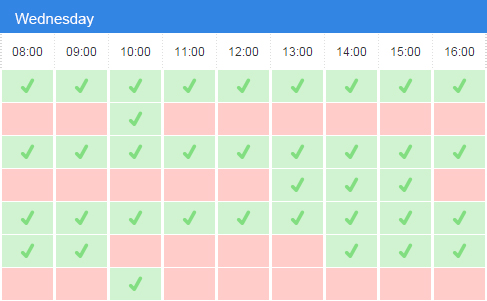
\includegraphics[scale=0.70]{fig/summary/wednesday}
    \caption{Example of our schedule. One row for each team member.}
    \label{fig:wednesday}
\end{figure}


\subsection{Abroad}
\noindent One of the group members had a part-time job in London the first half of the semester. This did not help the already troublesome schedule crash.
In addition, there was an excursion in March that three of the members were attending. This all meant a way of having stand-up meetings and exchanging information more frequently than the two meetings a week was needed. Geekbot was chosen for arranging online stand-up meetings. Communication is detailed in section \ref{sectionCommunicationTools}.

\subsection{Group member leaving}
At the beginning of the second iteration, a group member had to leave the course and the project for personal reasons. This meant that the group would go from seven people, down to six. The group worked around this by reassigning the workload to the remaining members. This announcement happened at a less unfortunate time, as the tasks for the second sprint had not yet been fully decided upon; planning for a six person group was relatively easy. 

This could of course have become problematic later on in the project if the total workload was larger than the reduced team could handle. Keeping in mind that the customer was more interested in a demonstration than the product features, scaling down functional requirements accordingly did not concern the customer much.

\section{Lessons learnt}

\subsection{Project organisation}

\paragraph{Schedules} Matching schedules is not a necessity for a project to succeed, but it makes the job a whole lot easier. Through planning and different tools, the problems were simplified, but with more similar schedules this could have been avoided in the first place. 

\paragraph{Development method} Looking back at the project, starting out with a more defined development method would have been beneficial and saved us some time. Agile development methods like Scrum work better when the team has a common background regarding development tools and how to use them. Digital Scrum boards, stand-up meetings, and other elements take time to learn and accustom to, and thus often benefit less than the required time investment for small projects.

\paragraph{Meetings} Even though it was not a huge problem, having more frequent meetings and work sessions would have improved the overall progression of the project early on. 

\subsection{Development}

\paragraph{Tools and frameworks} Learning to use tools and frameworks not familiar to the team may take more time than first anticipated. Thus, one should try to mostly use tools people are familiar with, unless the tool is required and there are no familiar alternatives.

\paragraph{Status} The status service could contain a cache of documentation and check if a newer version is available, to make sure documentation for a service is available even if the service is unavailable.

\paragraph{Front-end} The implemented front-end of the system is a bit too tightly coupled to be a true microservice. By splitting it up, or having different services provide their own front-end, this could have been achieved. This would require more work, despite being a nice possible addition to the project. 

\section{Conclusion}
The project started with some difficulties due to absence of one of the team members. This was handled by selecting an appropriate tool to facilitate team communication. This turned out to work quite well and had no major impact on the work flow. The roles and responsibilities of each team member were settled in a natural way, as each team member took on tasks that had been prioritised by the team. As the project evolved the different sub-teams worked on their part of the project and reported on the status during the weekly meetings. During the meetings people had the opportunity to share information and seek help on any problems encountered. 

Communication with the customer has been good overall, even though some more preparations could have been done beforehand by the team. All in all the project went smoothly and no major problems were encountered. 
%Any problems encountered along the way was taken care of in an efficient and effective way by the team, making the whole experience informative and interesting.

Even though the system is only a demonstration of microservices, it is a possibility that a third party might be interested in continuing working on the project. Therefore, steps have been taken to ensure that future developers can easily continue on the project if needed. The \acrshort{api} for every applicable microservice has been documented, so the services are easy to work with. If creating a replacement for a microservice is desirable, it is easy to find out which features require being implemented. A setup guide has been created to make it easy to deploy a new instance of the system. There are also tests for the services that can be used to validate future changes and make sure the system remains stable.

% forslag til oppsummerende setning: All in all the group felt that the requirements and goal defined at the start of the project ...somthing something ..

\section{Summary}

The project originated in the customer's expressed desire for a system implementation using microservices.
The group, through this project having implemented such a system, has to a large degree noticed many of the advantages that microservices are purported to have, which reflects many of the customer's hopes and expectations. %JA?
Overall, we feel that the requirements and goals outlined have been achieved to a satisfactory degree.


% Include more chapters as required.

%%=========================================
%  Biblography
\pagenumbering{roman}
\setcounter{page}{\thesavepage}
\bibliographystyle{apa}
\addcontentsline{toc}{chapter}{\bibname}
\bibliography{appendix/refs}

%%=========================================
%  Appendix
\appendix
\include{appendix/figures}
% !TEX encoding = UTF-8 Unicode
%!TEX root = thesis.tex
% !TEX spellcheck = en-US
%%=========================================




%% TODO give these a new id scheme since this is the same as the user stories ##########################
%% Also fix the problem with the commas (replace commas which are in the middle of text with {,} 
\begin{table}[p]
   % WTF OLEX WHY IS TEHRE A CHAPTER HERE???
   \chapter{Requirements} \label{requirements} % Should this be renamed? Best practise for appendix iiis?
   \section{Content module}
   \caption{Functional requirements for the content services}
   \centering
   \begin{tabular}{|p{1cm}|p{10cm}|p{4cm}|}\hline%
        ID & Description & Service\\\hline\hline
        \csvreader[late after line=\\\hline]%
        {tables/appendix/content_req.csv}{ID=\ID, Description=\Description, Service=\Service}%
        {\ID & \Description & \Service}%
    \end{tabular}
\end{table}


\clearpage
\section{Authentication module}
\begin{table}[H]
   \caption{Functional requirements for the authentication service}
   \centering
   \begin{tabular}{|p{1cm}|p{10cm}|p{4cm}|}\hline%
        ID & Description & Service\\\hline\hline
        \csvreader[late after line=\\\hline]%
        {tables/appendix/auth_req.csv}{ID=\ID, Description=\Description, Service=\Service}%
        {\ID & \Description & \Service}%
    \end{tabular}
\end{table}

\section{Search module}
\begin{table}[H]
   \caption{Functional requirements for the search service} 
   \centering
   \begin{tabular}{|p{1cm}|p{10cm}|p{4cm}|}\hline%
        ID & Description  Service\\\hline\hline
        \csvreader[late after line=\\\hline]%
        {tables/appendix/search_req.csv}{ID=\ID, Description=\Description, Service=\Service}%
        {\ID & \Description & \Service}%
    \end{tabular}
\end{table}

% This is wrong :'(
% \section{Test plans}
% \todo[inline]{Make subsections for each service when test plans are completed}

% \subsection{All}\label{appendix:testplans}
% Stored in Google Sheets for the time being for easy access, easy updating and referencing: \url{https://drive.google.com/open?id=1Oz8ldDk0ZnQiEJkNAxjlzAW2eUIXtuDXVDvkymlJj8c}.
% 
% \textit{Due to the fact that each of the services are developed by different teams, it's not possible for one of the developers to create a test plan for the system as a whole. Members of each of the sub-projects have to create plans for services when work on the service starts, and as not all services have started development, some test plans might be missing and/or incomplete.}
% 
% \begin{table}
%     \caption{Test plan: Microauth}
%     \label{table:testplan-microauth}
%     \centering
%     \begin{tabular}{| r | r | p{7.5cm} | c |}
%         \hline
%         Test Scenario ID & Req. & Description & Importance \\ \hline
%         MA-REG-1 & A-2 & It should be possible to sign up users according to the specified guidelines & High \\ \hline
%         MA-AUTH-1 & A-1 & Users should be able to log in & High \\ \hline
%         MA-PERM-1 & A-4 & Users should only be able to view content viewable by them according to their restrictions & Medium \\ \hline
%         MA-PERM-2 & A-5 & It should be possible to define different levels of restrictions and permission levels, so that users may be trusted to perform various actions based on the preferences of a system administrator & Medium \\ \hline
%     \end{tabular}
% \end{table}
% 
% \begin{table}
%     \caption{Test plan: Content}
%     \label{table:testplan-content}
%     \centering
%     \begin{tabular}{| r | r | p{9.5cm} | c |}
%         \hline
%         Test Scenario ID & Req. & Description & Importance \\ \hline
%         CT-CE-1 & CE-1 & Users should be able to open the editor, create an article and save it & High \\ \hline
%         CT-CE-2 & CE-2 & Users should be able to select a template to use. & Low \\ \hline
%         CT-CE-3 & CE-3 & Users should be able to select an image to insert,and resize it. & Medium \\ \hline
%         CT-CE-4 & CE-4 & Users should be able to select a file and add it. & Medium \\ \hline
%         CT-CD-1 & CD-2 & Users should be able to select what information to publish and publish it. & Medium \\ \hline
%         CT-CD-2 & CD-2 & Users should be able to download published calendar information, and open it in google calendar and Outlook. & Medium \\ \hline
%         CT-CA-1 & CA-2 & Users should be able to add elements to menus,and remove them. & Medium \\ \hline
%         CT-CP-1 & CP-1 & Users should be able to publish the content in the editor. & High \\ \hline
%         CT-CP-2 & CP-1 & Users should be able to select a file and publish it. & High \\ \hline
%         CT-CP-3 & CP-3 & Users should be able to set an expiration date for published content. & Low \\ \hline
%         CT-CP-4 & CP-3 & Content should become unavailable after its expiration date. & Low \\ \hline
%         CT-CP-5 & CP-4 & Users should be able to open metadata for a file and edit it. & Low \\ \hline
%         CT-CP-6 & CP-5 & Users should be able to chose to disable indexing when publishing a file. & Low \\ \hline
%         CT-CP-7 & CP-6 & Users should be able to inset a hyperlink in the content editor. & Medium \\ \hline
%         CT-CP-8 & CP-6 & Users should be taken to the chosen page when clicking on the hyperlink made in the editor. & Medium \\ \hline
%     \end{tabular}
% \end{table}
%% !TEX encoding = UTF-8 Unicode
%!TEX root = thesis.tex
% !TEX spellcheck = en-US
%%=========================================

\chapter{Changelog}
\todo[inline]{Decide on whether this chapter is neccessary}

\todo[inline]{Write about changes to requirements during development (some modules have not been implemented etc.). \\
{[}Prio:Medium-high{]}}
% !TEX encoding = UTF-8 Unicode
%!TEX root = thesis.tex
% !TEX spellcheck = en-US
%%=========================================

\chapter{Setup guide}
\section*{Initial requirements}
\begin{itemize}
    \item A server running Debian (Jessie or newer) with more than 2GB of RAM and 10GB of free space. The server should also have git installed.
    \item A domain pointing to the server mentioned above.
    \item SSL/TLS certificates for the domain mentioned above SSL/TLS is not required, but it is recommend as you would otherwise have to change some of the services.
    \footnote{Certificates can be obtained for free by following: \url{https://www.digitalocean.com/community/tutorials/how-to-secure-nginx-with-let-s-encrypt-on-ubuntu-14-04}}
    \item Prior experience with Linux and the command line.
\end{itemize}

\section*{Step 1 - Installing the required software}
Begin by installing docker, docker-compose and nginx, which is required to run the system..
If the server is running Debian Jessie, you must first add the Debian Stretch package repository, as Nginx 1.10 or newer is required.
\clearpage % As the command below would otherwise be split between two pages and a footnote(!).
The Stretch package repository can be used by adding:
\begin{verbatim}
    deb http://http.debian.org/debian stretch main
\end{verbatim}
to /etc/apt/sources.list, and then running:
\begin{verbatim}
    apt-get update
\end{verbatim}
in order to obtain the packages from the newly added repository.
Nginx is then installed by running:
\begin{verbatim}
    apt-get -t stretch install nginx-extras
\end{verbatim}
or just
\begin{verbatim}
    apt-get install nginx-extras
\end{verbatim}
if you are running a newer version than Jessie.

After having installed Nginx, follow:
\begin{itemize}
    \item \url{https://docs.docker.com/engine/installation/linux/debian/}
    \item \url{https://docs.docker.com/compose/install/}
    \item \url{https://github.com/jwilder/docker-gen}
\end{itemize}
to install docker, docker-compose and docker-gen.


\section*{Step 2 - Adding configuration files}
Begin by running:
\begin{verbatim}
    git clone https://github.com/microserv/deploy
\end{verbatim}
to obtain the configuration files needed to deploy the system.

Now enter the newly created \textit{deploy} folder, and replace all references to \textit{despina.128.no} with your own domain name.
This can also be done by executing the following command:
\begin{verbatim}
    find . -type f -exec sed -i 's/despina.128.no/<YOUR DOMAIN HERE>/g' {} +
\end{verbatim}
Then, copy the docker-gen configuration file \textit{deploy/docker-gen/docker-gen.cfg} to \textit{/etc/} and the docker-gen systemd unit file \textit{deploy/docker-gen/docker-gen.service} to \textit{/etc/systemd/system}.

After copying the files mentioned above, copy the nginx configuration file \textit{deploy/nginx/nginx.conf} to \textit{/etc/nginx/} and the nginx docker-gen template \textit{deploy/docker-gen/nginx.conf.tmpl} to \textit{/etc/nginx/}

Now enable the docker-gen systemd unit file by running:
\begin{verbatim}
    systemctl daemon-reload
    systemctl start docker-gen
\end{verbatim}

\section*{Step 3 - Launching the system}
The system is launched using docker-compose. Docker-compose automatically fetches the Docker images required to launch the containers. The Docker images is by default fetched by Docker from a private repository hosted at 128.no:8080. To be able to access this repository, you must first log-in. To log-in execute:
\begin{verbatim}
    docker login dockerisfun:QRN5A2So
\end{verbatim}

Now enter the \textit{deploy/docker} folder, and run:
\begin{verbatim}
    docker-compose -d
\end{verbatim}
to launch the system.

The system should be running and accessible through your domain after about 15 seconds. Then, access the administration panel by first accessing \textit{YOUR-DOMAIN-HERE/auth/admin} and logging in using \textit{admin} as the username, and \textit{aStupidDefaultPasswordYouShouldChange} as the password.

After having logged in, go to \textit{Applications}, then \textit{Publishing}, and replace despina.128.no with your own domain in the \textit{redirect URI} field. The system should now work as intended.

Kibana, elasticsearch and logstash, which is used to monitor the logs produced by the Docker containers can be launched by running the script \textit{start-docker-logging.sh} in the \textit{docker} folder. These services can be stopped by running \textit{stop-docker-logging.sh} in the same folder. When these services are up, the logs can by read by accessing \textit{YOURDOMAINNAMEHERE/kibana/}.
% !TEX encoding = UTF-8 Unicode
%!TEX root = thesis.tex
% !TEX spellcheck = en-US
%%=========================================


\chapter{User manual}
The core functionality of the system is to create and view articles. All main functionality is accessible through the main menu on top of the screen. 


%% #################  Article  ##################
\section{Creating an article}
\paragraph{Step 1:} In order to create an article, you will need to go to the editor page. Click the editor button as marked in \ref{fig:manual1}. If you are signed in and authorised, go to step 3, if not, continue to step 2.

\begin{figure}[H]
    \centering
    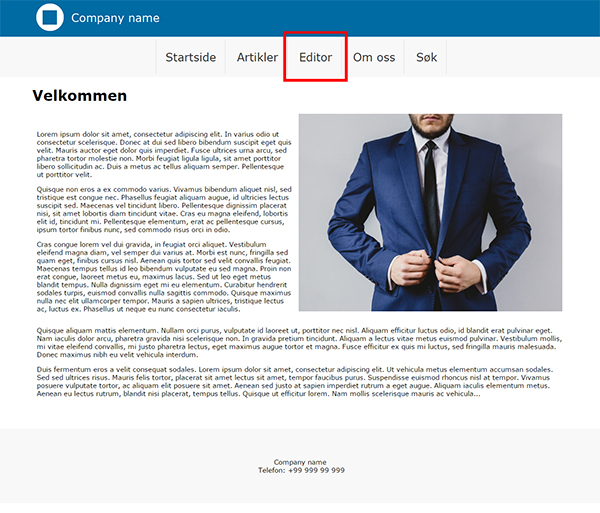
\includegraphics[scale=0.70]{fig/userManual/1}
    \caption{Showing location of the editor button in main menu}
    \label{fig:manual1}
\end{figure}


\paragraph{Step 2:} Fill in your credentials and log in as shown in figure \ref{fig:manual2}. This will prompt you with an authorisation screen. Click "Authorize" in order to get access (displayed in figure \ref{fig:manual3}).

\begin{figure}[H]
    \centering
    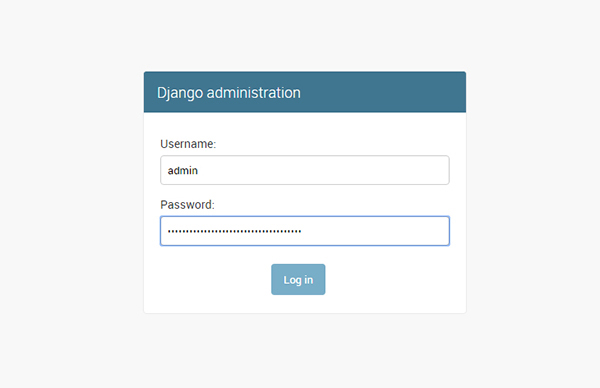
\includegraphics[scale=0.70]{fig/userManual/2}
    \caption{View for step 2}
    \label{fig:manual2}
\end{figure}

\begin{figure}[H]
    \centering
    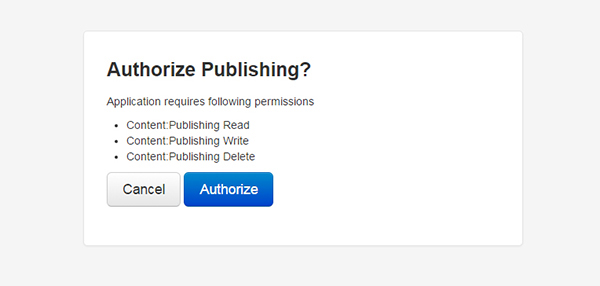
\includegraphics[scale=0.70]{fig/userManual/3}
    \caption{View for step 2}
    \label{fig:manual3}
\end{figure}

\paragraph{Step 3:} You will then need to choose which template you want to base your article on from the drop down list titled "Velg en mal".

\begin{figure}[H]
    \centering
    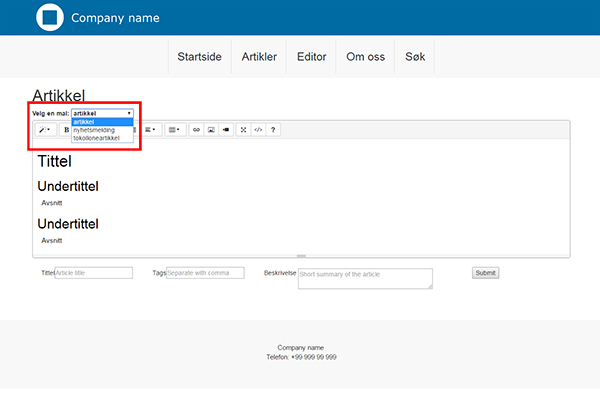
\includegraphics[scale=0.70]{fig/userManual/4}
    \caption{Showing location of the template drop-down list}
    \label{fig:manual4}
\end{figure}


\paragraph{Step 4:} Once you are done writing the article and adding metadata like title and description, you submit it by clicking the "submit"-button in the bottom-right corner. 
\begin{figure}[H]
    \centering
    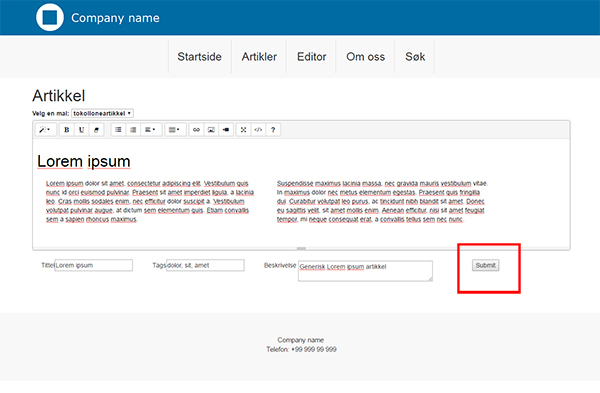
\includegraphics[scale=0.70]{fig/userManual/5}
    \caption{Showing location of the submit button}
    \label{fig:manual5}
\end{figure}


%% #################  Search  ##################
\section{Searching}
Articles can be found in two ways; either by finding them in the article list, as shown in figure \ref{fig:manual6}, or by searching. The following steps explain how to use the search function.

\begin{figure}[H]
    \centering
    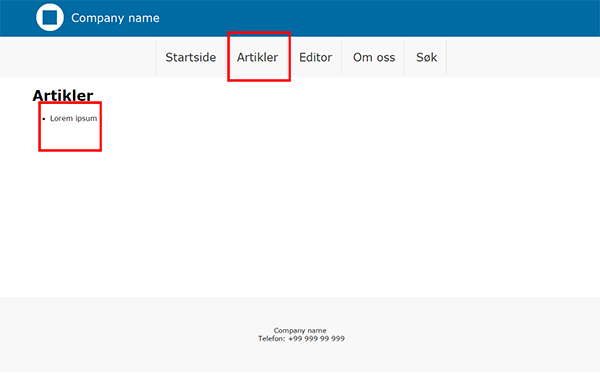
\includegraphics[scale=0.70]{fig/userManual/6}
    \caption{Showing location of the submit button}
    \label{fig:manual6}
\end{figure}

\paragraph{Step 1:} First, go to the search page as show in figure \ref{fig:manual7}.

\begin{figure}[H]
    \centering
    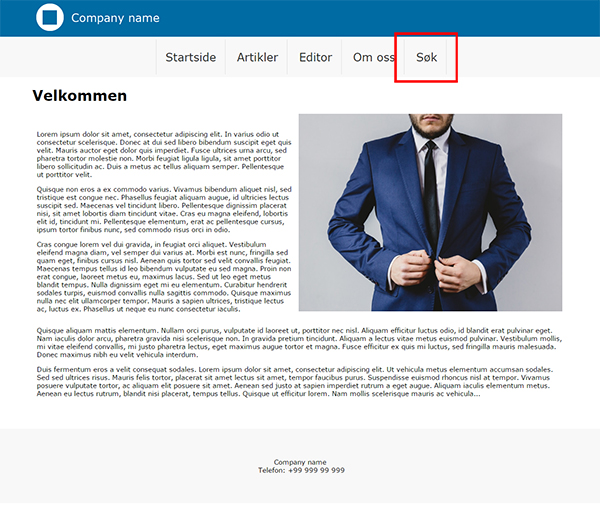
\includegraphics[scale=0.70]{fig/userManual/7}
    \caption{Showing location of the search button in main menu}
    \label{fig:manual7}
\end{figure}


\paragraph{Step 2:} When you start writing in the search field, it will give you suggestions of completions for potentially incomplete words. In order to accept this suggestion you can either left-click it or press the down-arrow on your keyboard. 

\begin{figure}[H]
    \centering
    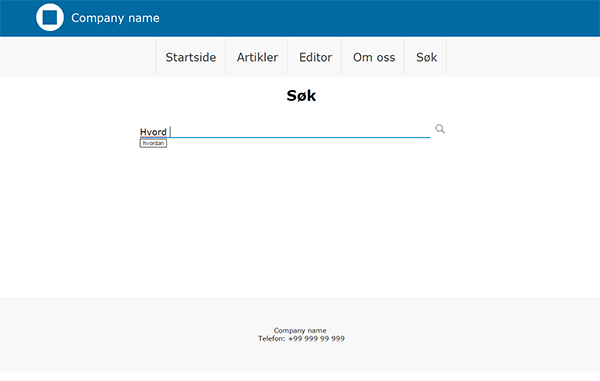
\includegraphics[scale=0.70]{fig/userManual/8}
    \caption{Word completion suggestion}
    \label{fig:manual8}
\end{figure}

\paragraph{Step 3:} Once your query is completed, you can search by either clicking the search icon or pressing the return key on your keyboard. This will present you with a suggestion to spelling in your query, which can be accepted the same way as suggestions in step 2. It will also present you with potential results, as shown in figure \ref{fig:manual9}.

\begin{figure}[H]
    \centering
    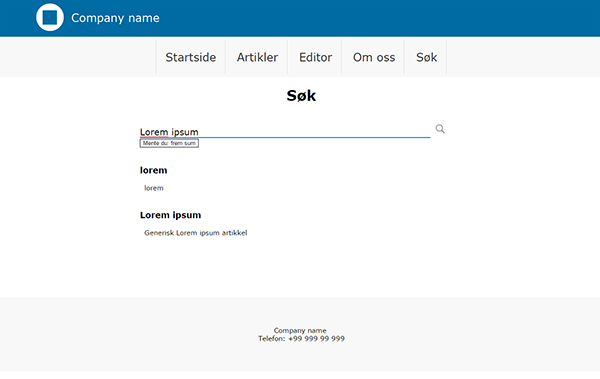
\includegraphics[scale=0.70]{fig/userManual/9}
    \caption{Search results}
    \label{fig:manual9}
\end{figure}

\paragraph{Step 4:} By clicking the article title you are brought to the full article as shown in figure \ref{fig:manual10}

\begin{figure}[H]
    \centering
    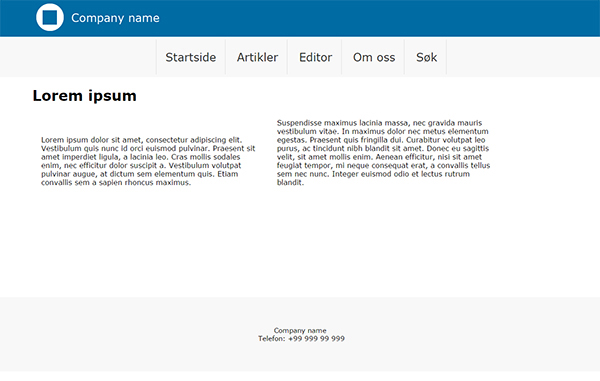
\includegraphics[scale=0.70]{fig/userManual/10}
    \caption{Full article}
    \label{fig:manual10}
\end{figure}




%% #################  Status  ##################
\section{Viewing service status}

\paragraph{Step 1:} Seeing as status is a developer feature, it is not clearly indicated with a button. In order to access it you need to click "Om oss" in the menu and then "Service status overview", as shown in figure \ref{fig:manual14}.

\begin{figure}[H]
    \centering
    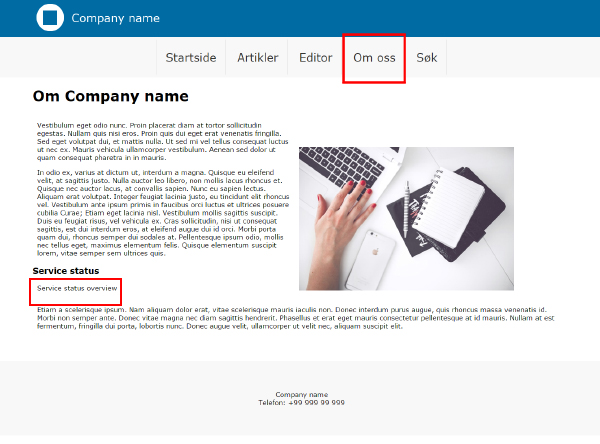
\includegraphics[scale=0.70]{fig/userManual/14}
    \caption{Hidden status button}
    \label{fig:manual14}
\end{figure}

\paragraph{Step 2:} By clicking 'show' on any of the services, you are provided extra information about its status. An example of the view for the indexer service can be seen in figure \ref{fig:manual11}.

\begin{figure}[H]
    \centering
    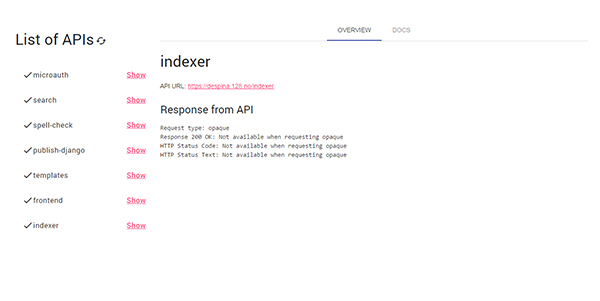
\includegraphics[scale=0.70]{fig/userManual/11}
    \caption{Status overview. The symbol in front of the name represents its state. Check mark means available and an error symbol means it's unavailable.}
    \label{fig:manual11}
\end{figure}
% The status of each service is indicated by a symbol in front of its name. A check mark indicates that its running, a spinner shows when it is querying the service and an error symbol when it's unavailable. 

\paragraph{Step 3:} For viewing the documentation for the service, click on "Docs" in the upper-right corner as highlighted in figure \ref{fig:manual12}.

\begin{figure}[H]
    \centering
    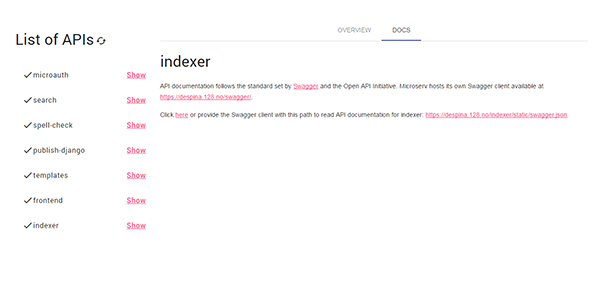
\includegraphics[scale=0.70]{fig/userManual/12}
    \caption{Service documentation}
    \label{fig:manual12} 
\end{figure}


%%=========================================

\end{document}
